\documentclass[12pt,a4paper]{article}

% --- Пакеты ---
\usepackage[utf8]{inputenc}
\usepackage[T2A]{fontenc}
\usepackage[russian]{babel}
\usepackage{amsmath, amssymb, amsfonts}
\usepackage{graphicx}
\usepackage{geometry}
\usepackage{booktabs}
\usepackage{hyperref}
\usepackage{float}
\usepackage{caption}
\usepackage{subcaption}

\geometry{left=2.5cm,right=1.5cm,top=2cm,bottom=2cm}

% Путь к папке с рисунками
\graphicspath{{figures/}}

\title{\textbf{Исследование однопараметрического семейства периодических орбит Ляпунова\\ в плоской задаче трёх тел с равными массами}}
\author{}
\date{}

\begin{document}

\maketitle

\section{Введение и постановка задачи}

Рассматривается плоская задача трёх тел с равными массами \(m_1 = m_2 = m_3 = 1\) и гравитационной постоянной \(G = 1\). Исследуется однопараметрическое семейство периодических орбит (Ляпунова), ответвляющееся от эйлеровой коллинеарной конфигурации. В равновесии расстояния между телами равны 1, а система вращается с угловой скоростью \(\Omega = \sqrt{5/4}\).

Работа опирается на два набора данных, содержащих численно продолженные орбиты:
\begin{enumerate}
    \item \texttt{catalog\_unified.tsv} — 16\,128 орбит, разделённых на три блока (\textit{canonical}, \textit{near\_bif}, \textit{long}). Параметром продолжения в первых двух блоках служит начальное значение \(A = y_1(0)\) (в координатах Якоби), а в блоке \textit{long} — параметр в декартовых координатах. Состояния в этом каталоге уже повёрнуты на угол \(-\theta\).
    \item \texttt{catalog\_arclength.txt} — 83\,461 орбита. Параметром продолжения является псевдо-длина дуги в фазовом пространстве \((X, T)\). Состояния записаны в декартовых координатах без дополнительного поворота.
\end{enumerate}
Важно отметить, что с физической точки зрения каталоги описывают одно и то же семейство; различие в параметризации не вносит разрыва в физику орбит, а лишь меняет шаг продолжения.

Для интегрирования уравнений движения использовался высокоточный интегратор \texttt{heyoka} (метод Тейлора, тип данных \texttt{real128}, допуск \(\text{tol} = 10^{-25}\)). Для орбит с экстремально глубокими сближениями (\(d_{\min} < 10^{-7}\)) точность повышалась до 256 и более бит. Периодичность орбит уточнялась методом Ньютона для решения краевой задачи \(X(T; X_0) = X_0\).

\section{Методы и инструментарий}

\subsection{Спектральный анализ}
Устойчивость периодических орбит исследуется с помощью матрицы монодромии \(M\), которая получается интегрированием уравнений в вариациях за один период \(T\). Собственные значения \(\mu\) матрицы \(M\) называются мультипликаторами Флоке. В гамильтоновых системах они обладают свойством симметрии: если \(\mu\) — мультипликатор, то \(\mu^{-1}\), \(\bar{\mu}\) и \(\bar{\mu}^{-1}\) также являются мультипликаторами.

Все орбиты в каталогах классифицируются по спектру на три типа:
\begin{itemize}
    \item \textbf{C} — четыре тривиальных мультипликатора \(\mu \approx 1\) и две комплексно-сопряжённые пары вне единичной окружности;
    \item \textbf{R} — четыре тривиальных мультипликатора и четыре вещественных мультипликатора, образующих две пары \((\mu, 1/\mu)\);
    \item \textbf{OTHER} — четыре тривиальных мультипликатора, одна комплексная пара и одна вещественная пара.
\end{itemize}
Показатель Ляпунова определяется как \(\lambda = \frac{1}{T} \ln(\max |\mu|)\).

\subsection{Пространство форм и поверхность нулевой скорости}
Для визуализации и анализа топологии относительного движения вводится координатное пространство \(\xi = (\xi_1, \xi_2, \xi_3)\), основанное на векторах Якоби. Пусть \(Q_1 = r_2 - r_1\) и \(Q_2 = r_3 - \frac{m_1 r_1 + m_2 r_2}{m_1 + m_2}\). Тогда координаты определяются как:
\begin{equation}
    \xi_1 = \mu_1 |Q_1|^2 - \mu_2 |Q_2|^2, \quad
    \xi_2 + i\xi_3 = 2\sqrt{\mu_1 \mu_2} \, Q_1 \overline{Q_2}.
\end{equation}
где \(\mu_1 = \frac{m_1 m_2}{m_1+m_2}\), \(\mu_2 = \frac{m_3(m_1+m_2)}{m_1+m_2+m_3}\). В этих координатах точка равновесия имеет вид \(\xi_{eq} = (-1, \sqrt{3}, 0)\), а момент инерции выражается как \(I = |\xi| = \sqrt{\xi_1^2 + \xi_2^2 + \xi_3^2}\).

Поверхность нулевой скорости (ZVS) в координатах \(\xi\) задаётся уравнением Сундмана:
\begin{equation}
    V(\xi) + \frac{L_z^2}{2|\xi|} = h_{in},
\end{equation}
где \(V(\xi)\) — потенциал, \(L_z\) — полный момент импульса, \(h_{in}\) — полная энергия в инерциальной системе. Область, где левая часть меньше \(h_{in}\), является доступной для движения.

\section{Спектральная структура и бифуркации}

В этом разделе исследуется эволюция спектра мультипликаторов Флоке вдоль семейства орбит. Показано, что топология спектра претерпевает качественные изменения, которые, однако, не всегда сопровождаются изменением устойчивости.

\subsection{Общая карта спектров и показателя Ляпунова}
В зависимости от расположения мультипликаторов на комплексной плоскости все орбиты в исследуемом семействе делятся на три класса: C, R и OTHER (см. раздел 2). 
На рисунке~\ref{fig:lambda_T_kind} показана зависимость показателя Ляпунова \(\lambda = \ln(\max |\mu|) / T\) от периода \(T\), раскрашенная по типу спектра. Видно, что орбиты типа C и R занимают непересекающиеся области, а тип OTHER (характерный для блока \textit{canonical} и начала \textit{near\_bif}) плавно переходит в них. Показатель \(\lambda\) монотонно убывает вдоль семейства от \(\approx 1.95\) (в начале блока \textit{canonical}) до \(\approx 0.3\) (в блоке \textit{arclength}).

\begin{figure}[H]
    \centering
    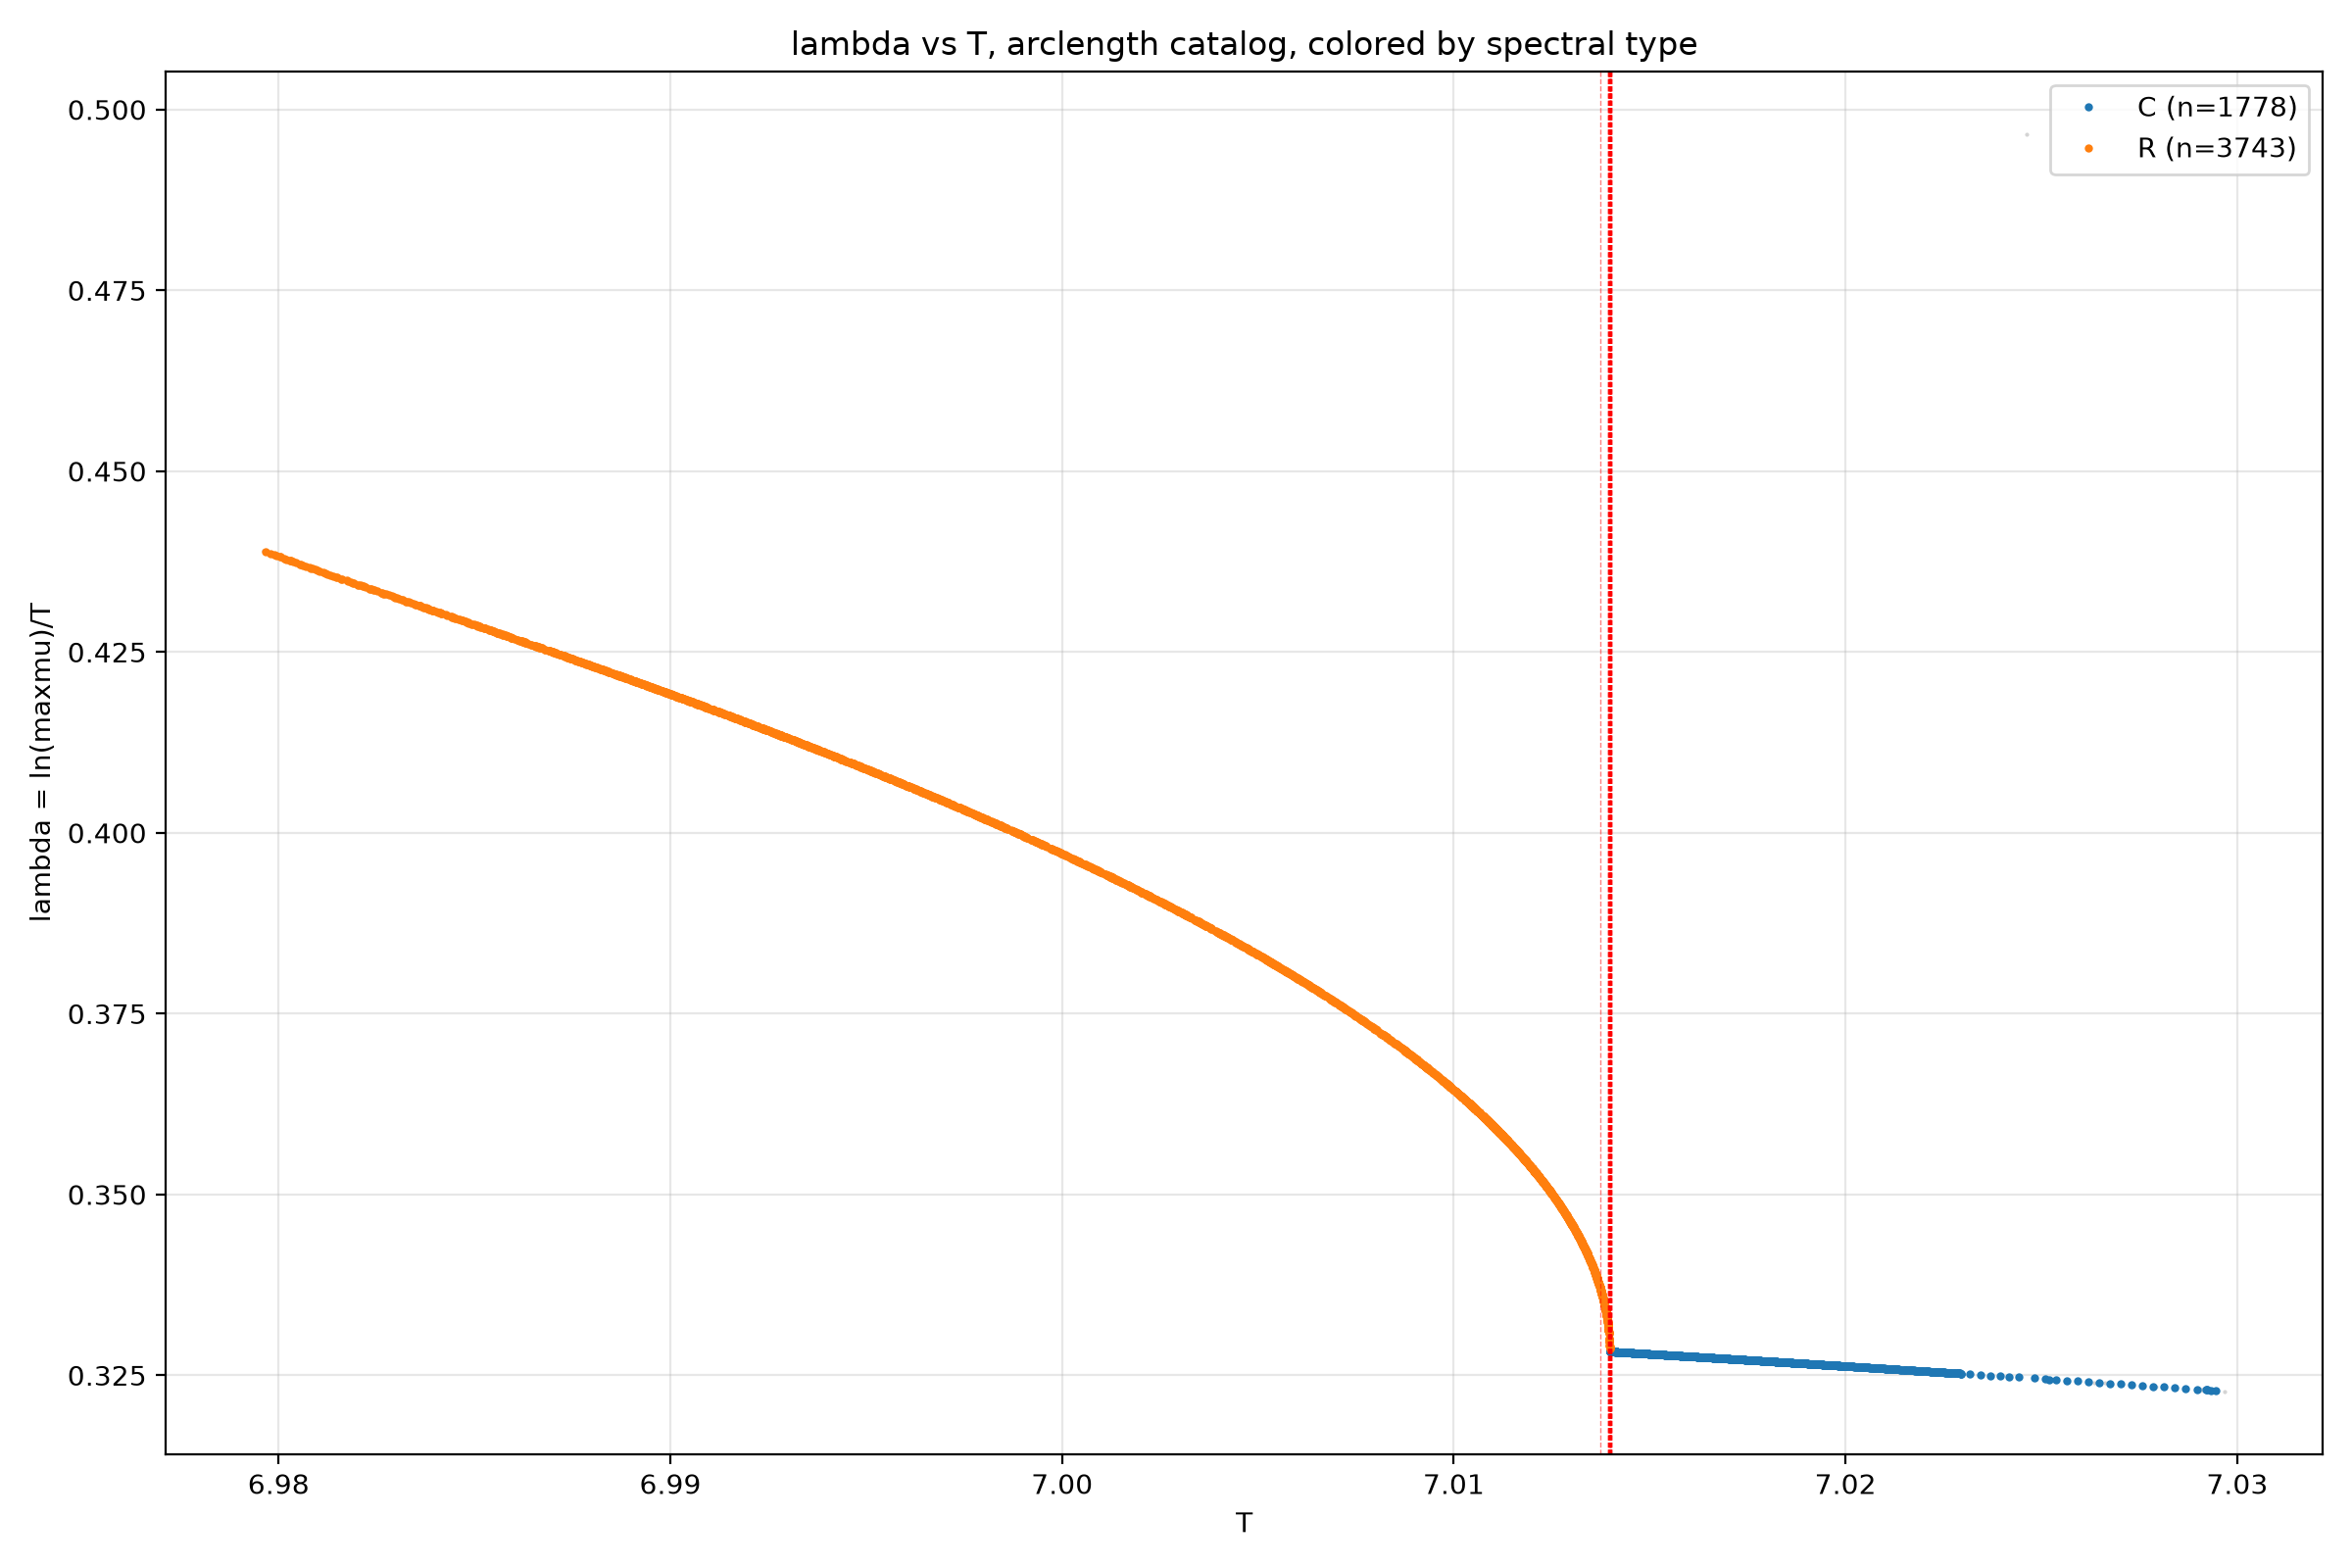
\includegraphics[width=0.85\textwidth]{30_lambda_T_kind.png}
    \caption{Зависимость показателя Ляпунова \(\lambda\) от периода \(T\). Цветом обозначен тип спектра (C, R, OTHER).}
    \label{fig:lambda_T_kind}
\end{figure}

\subsection{Единственное окно устойчивости в блоке unified}
В каталоге \texttt{catalog\_unified.tsv} было найдено единственное окно устойчивости, в котором все восемь мультипликаторов Флоке лежат на единичной окружности (т.е. \(\max |\mu| = 1\)). Это окно соответствует индексам \(gidx \in [15690, 15767]\) (периоды \(T \in [6.852, 6.989]\)).

Вход в это окно сопровождается переходом типа OTHER \(\to\) C. При \(gidx = 15690\) происходит следующее: вещественная пара мультипликаторов подходит к точке \(\mu = +1\), сливается с комплексной парой и обе уходят на единичную окружность. Этот процесс известен как \textbf{1:1 резонанс} или \textbf{столкновение Крейна} (Krein collision). 

Структура Жордана для мультипликатора \(\mu=1\) во всём семействе (кроме самой точки равновесия \(gidx=0\)) имеет вид \(J_2 + J_2\) (две жордановы клетки размера 2). Это стандартная структура для однопараметрического семейства в гамильтоновой системе, указывающая на отсутствие скрытых симметрий, порождающих дополнительную кратность. Точный переход OTHER \(\to\) C показан на рисунке~\ref{fig:other_c_transition}.

\begin{figure}[H]
    \centering
    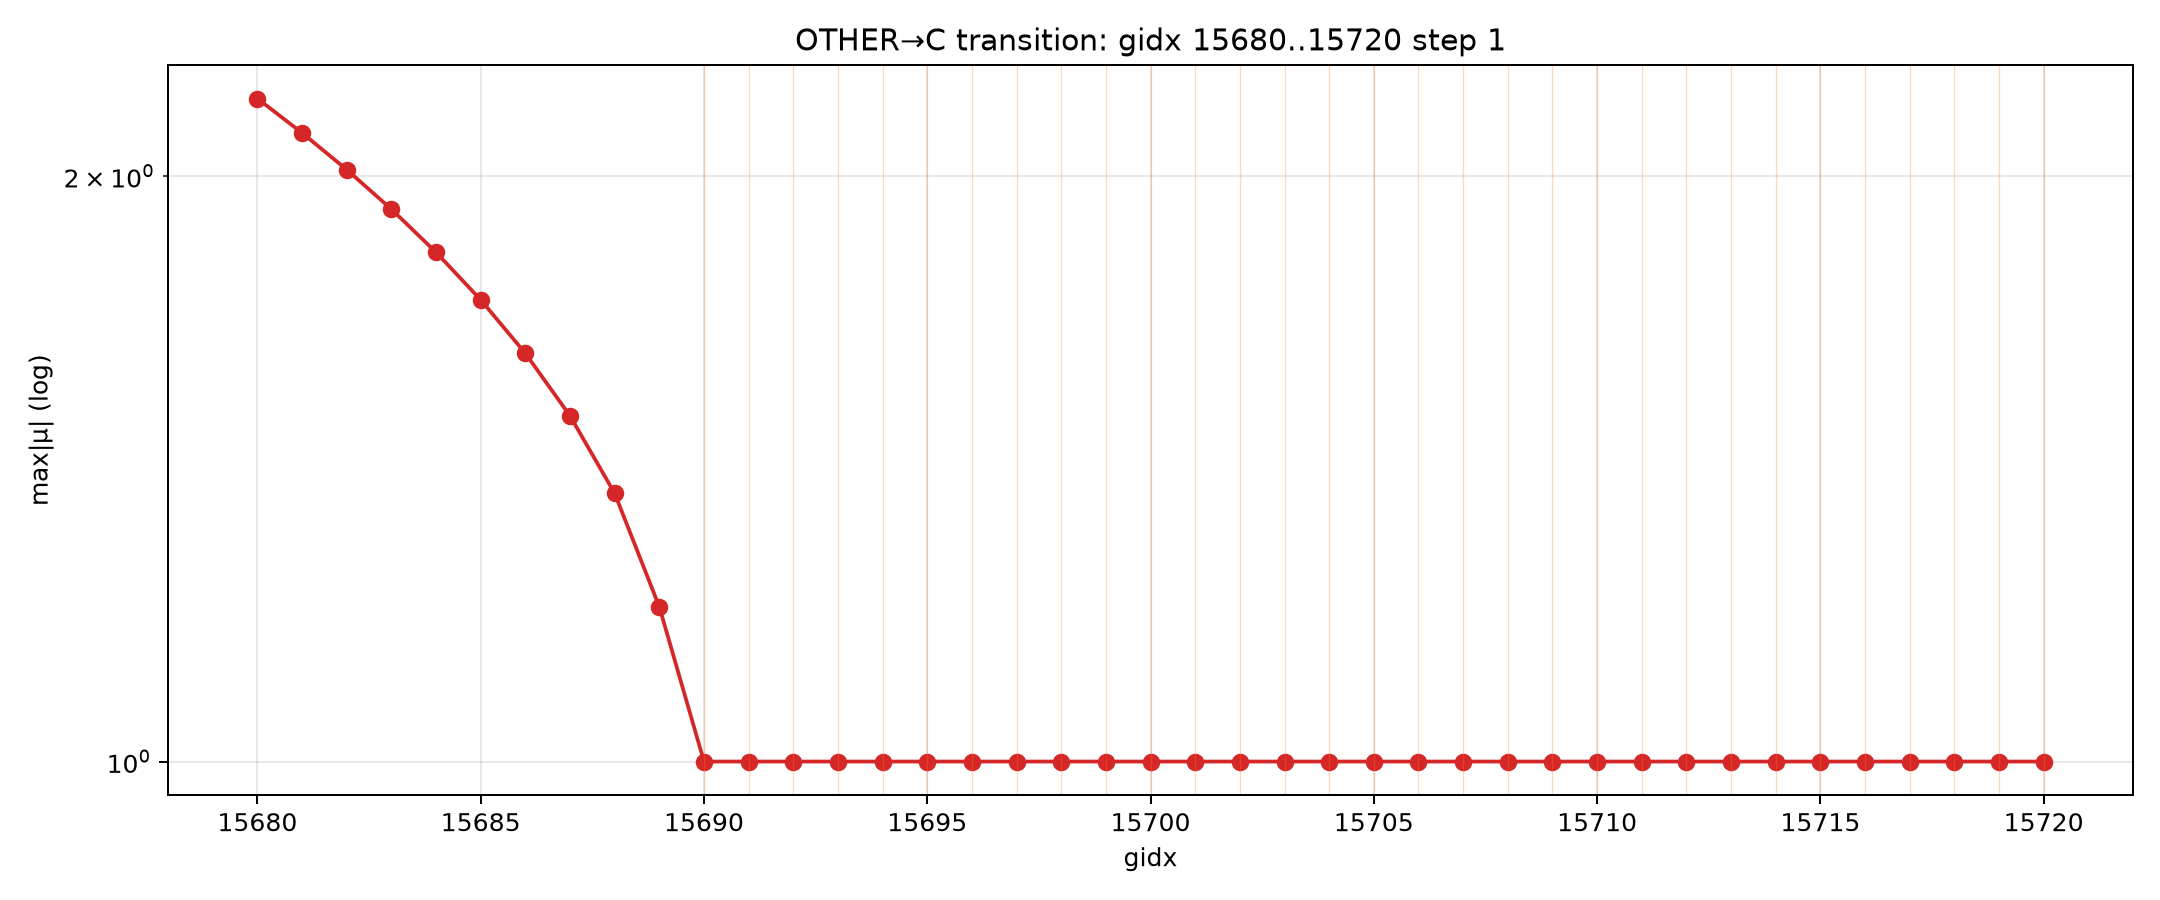
\includegraphics[width=0.85\textwidth]{88_other_c_transition.png}
    \caption{Точный переход OTHER \(\to\) C в блоке \textit{long} при \(gidx = 15690\) (1:1 резонанс) и последующее окно устойчивости.}
    \label{fig:other_c_transition}
\end{figure}

\subsection{Переходы C \(\leftrightarrow\) R в блоке arclength}
В блоке \textit{arclength} было зафиксировано 14 C-окон и 13 R-окон, которые строго чередуются. Всего найдено 27 переходов C \(\leftrightarrow\) R. 

Механизм всех этих переходов одинаков: пара комплексно-сопряжённых мультипликаторов с модулем \(\approx 0.100\) движется по комплексной плоскости, при подходе к вещественной оси их мнимая часть обращается в нуль, и они образуют вещественную пару \((\mu, 1/\mu)\). При этом \textbf{устойчивость орбиты не меняется}: показатель \(\lambda\) остаётся непрерывным, меняется лишь топология расположения мультипликаторов. В блоке \textit{long} (unified) переходов C \(\leftrightarrow\) R нет.

\subsection{Критический показатель \(\beta = 1/2\)}
Для количественного описания перехода C \(\leftrightarrow\) R рассмотрим поведение мнимой части мультипликатора вблизи точки бифуркации \(idx_c\). Было проверено 25 границ перехода. Для 17 из них линейная зависимость
\begin{equation}
    \text{Im}(\mu)^2 = a \cdot |idx - idx_c|
\end{equation}
выполняется с коэффициентом детерминации \(R^2 > 0.99\). Это подтверждает критический показатель \(\beta = 1/2\), характерный для слияния двух собственных значений на вещественной оси (седло-узловая бифуркация в терминах мультипликаторов). Результат линеаризованного коллапса показан на рисунке~\ref{fig:beta_collapse}.

\begin{figure}[H]
    \centering
    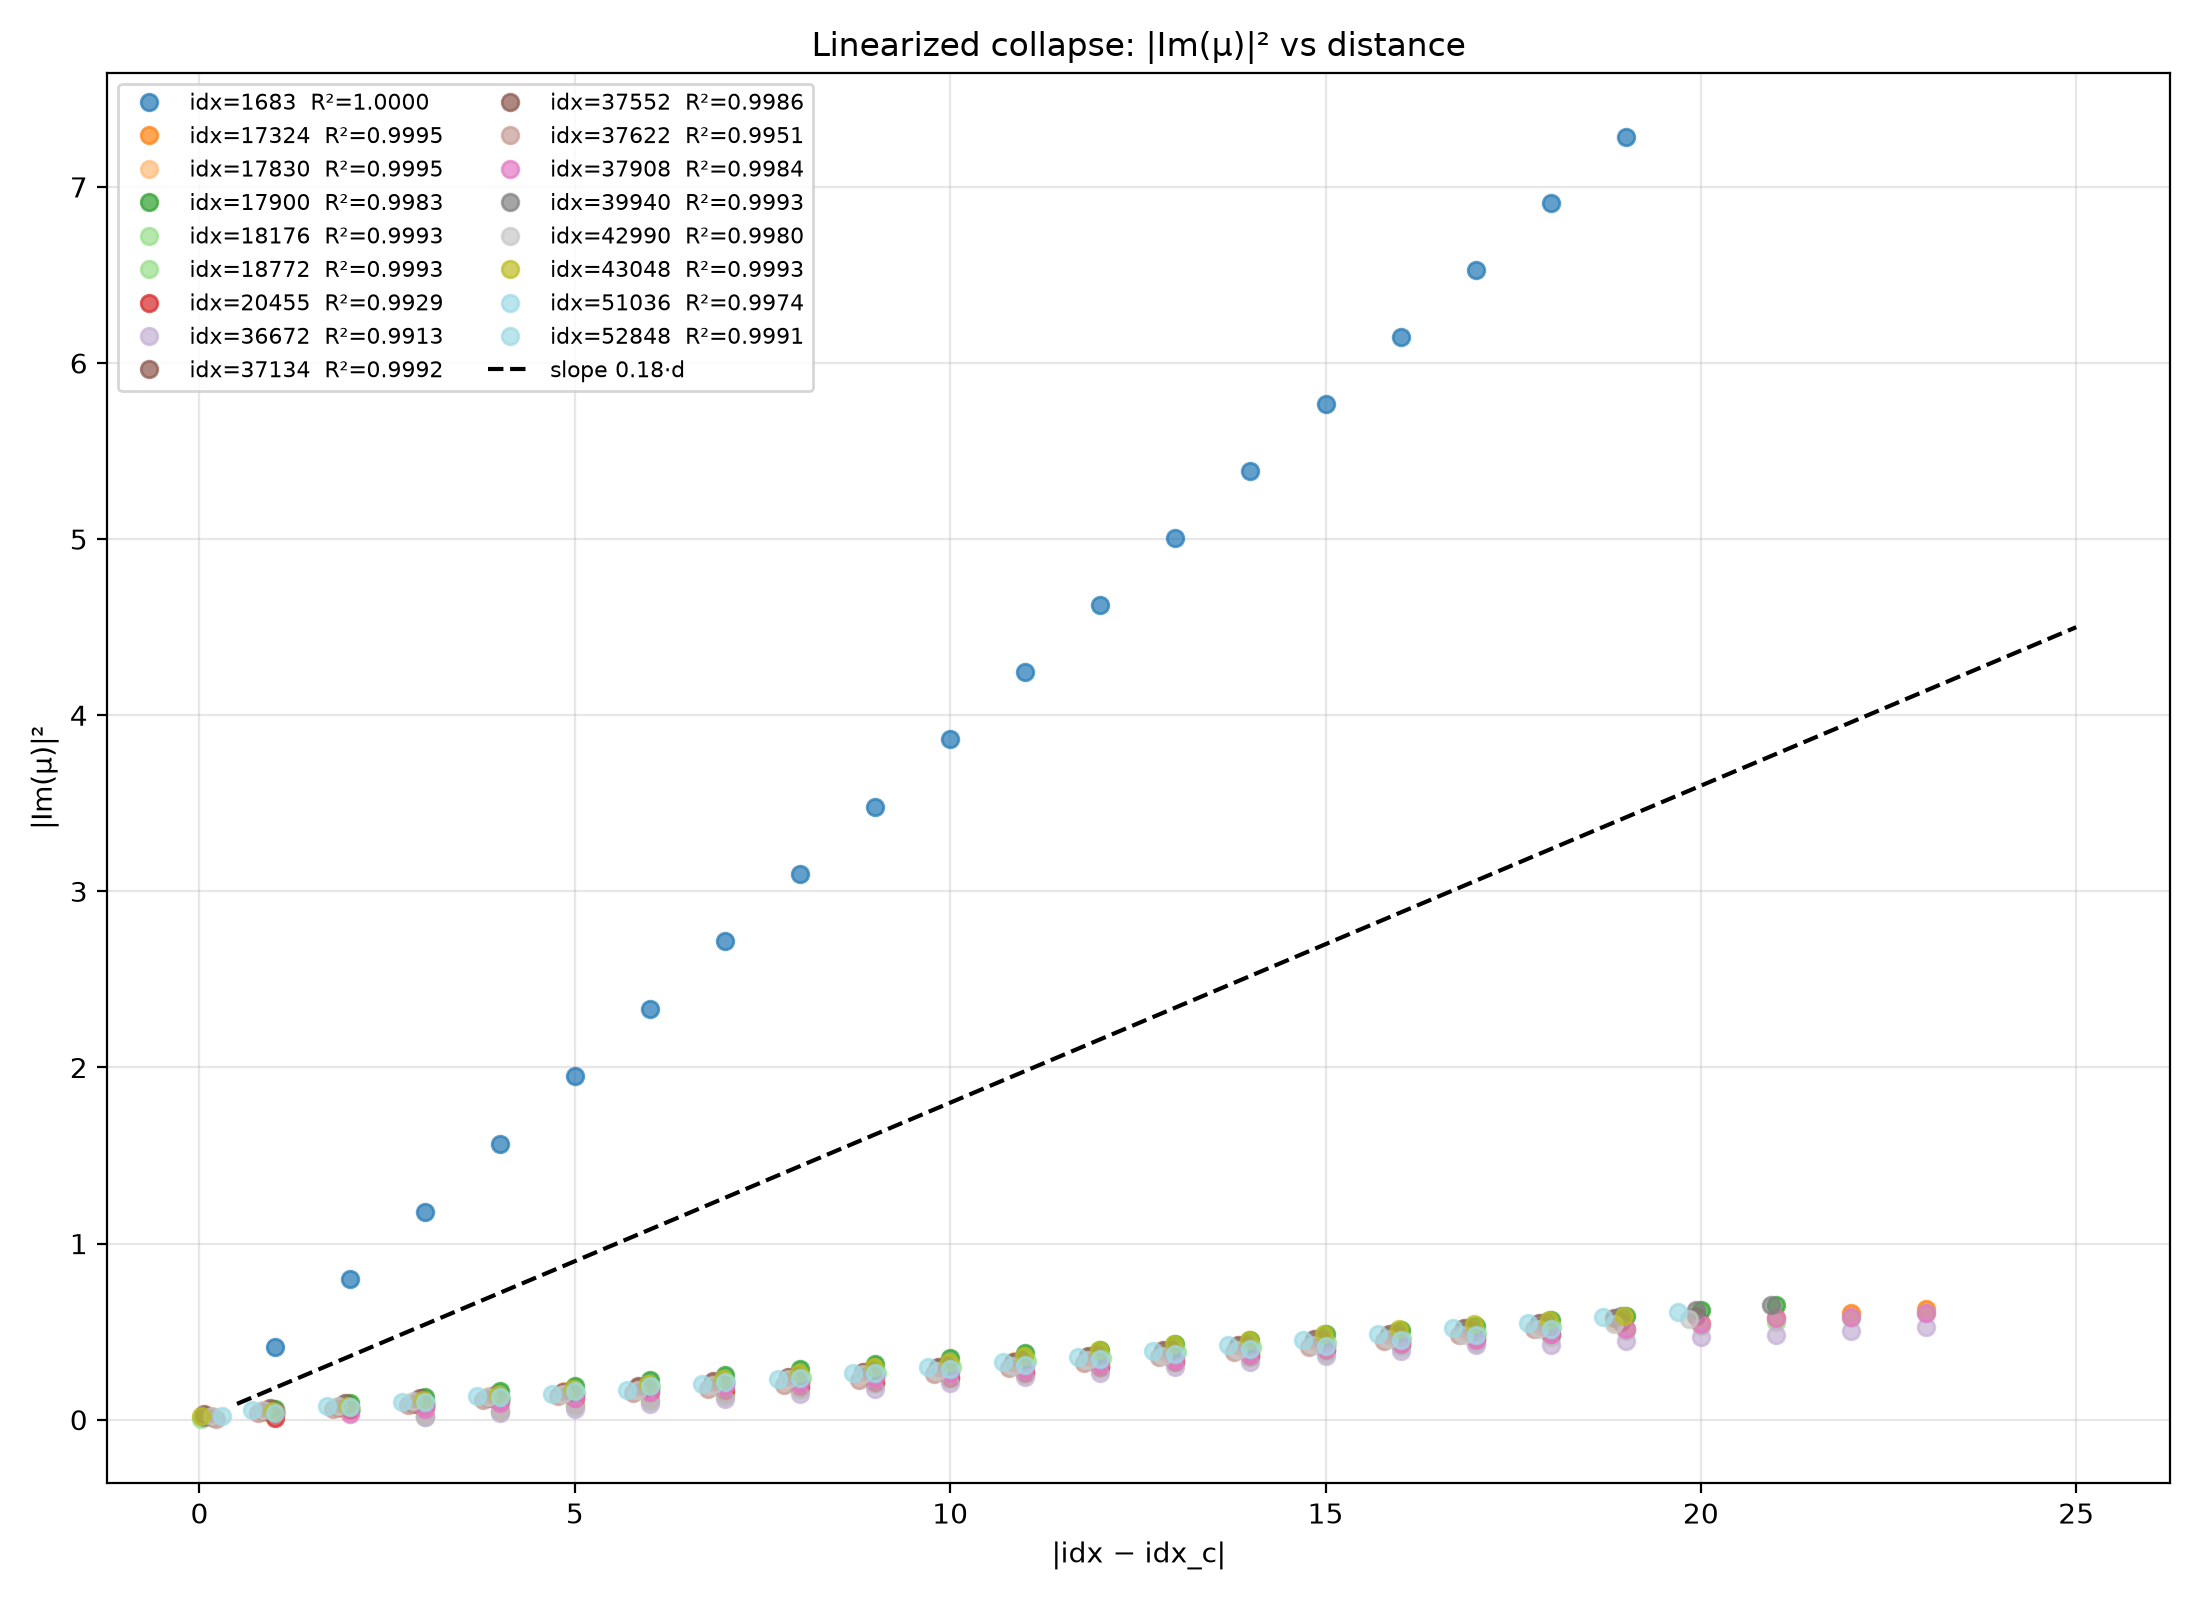
\includegraphics[width=0.8\textwidth]{39_linearized_collapse.png}
    \caption{Линеаризованный коллапс \(\text{Im}(\mu)^2\) от расстояния до точки перехода \(|idx - idx_c|\) для 17 границ C\(\leftrightarrow\)R. Наклон прямых соответствует \(\beta = 1/2\).}
    \label{fig:beta_collapse}
\end{figure}

\section{Устойчивость и медленная динамика}

В предыдущем разделе было показано, как меняется топология спектра Флоке. Теперь рассмотрим, как количественно меняется скорость неустойчивости (показатель Ляпунова \(\lambda\)) и какая геометрическая или динамическая характеристика орбиты за это отвечает.

\subsection{Связь показателя Ляпунова с геометрией}
Как было отмечено ранее, показатель \(\lambda = \ln(\max |\mu|)/T\) монотонно убывает вдоль семейства орбит примерно в 6 раз: от \(\lambda \approx 1.95\) в блоке \textit{canonical} до \(\lambda \approx 0.3\) в блоке \textit{arclength}. 

Первоначально возникает гипотеза о том, что эта скорость спада определяется просто периодом \(T\) (то есть \(\lambda \propto T\)). Однако при детальном анализе выясняется, что в плоскости \((T, \lambda)\) траектория семейства образует петли, и монотонной функции \(\lambda(T)\) не существует. 

Оказалось, что гораздо лучшим предиктором является геометрическая характеристика орбиты, названная \textbf{mean\_dev} (среднее отклонение от оси):
\begin{equation}
    \text{mean\_dev} = \frac{1}{T} \int_0^T \sqrt{\sin^2\theta_1 + \sin^2\theta_2} \, dt,
\end{equation}
где \(\theta_1\) и \(\theta_2\) — углы векторов \(\rho_1\) и \(\rho_2\) (расстояний в координатах Якоби) к оси \(X\). По сути, это средняя скорость отклонения тел от коллинеарной конфигурации (оси \(X\)) за период.

На выборке из 208 орбит (41 из \textit{unified} и 167 из \textit{arclength}) была построена линейная регрессия. Корреляция между \(\lambda\) и \textit{mean\_dev} оказалась равной \(r = -0.994\). Если исключить влияние \(T\), частичная корреляция остается \(r = -0.926\). Коэффициент детерминации для модели \(\lambda = a \cdot \text{mean\_dev} + b\) составил \(R^2 = 0.9888\). Это означает, что неустойчивость почти полностью определяется тем, насколько сильно орбита «отклоняется» от оси коллинеарности в среднем за период.

\subsection{Опровержение резонанса 5/4}
В ходе исследования возникла изящная гипотеза о том, что семейство орбит в блоке \textit{arclength} захватывается резонансом 5/4. Действительно, отношение периода орбиты к периоду вращения системы \(T / T_{rot}\) имеет медианное значение \(1.2452\), что всего на \(0.4\%\) отличается от \(5/4 = 1.25\). Кроме того, вход в блок \textit{arclength} происходит при \(idx=1593\), где \(T \approx 7.0252\), что почти совпадает с \(5 \pi / (2\Omega) \approx 7.0248\).

Однако эта гипотеза была отвергнута по двум причинам:
\begin{enumerate}
    \item В блоке \textit{arclength} величина \textit{mean\_dev} меняется всего на \(0.016\), а \(T\) — в пределах \(\pm 0.02\). Этот узкий диапазон создает иллюзию «плато» на графике \(T\) от параметра, в то время как на самом деле функция \(T(\text{mean\_dev})\) монотонно возрастает и не имеет полки, характерной для захвата в резонанс.
    \item Отношение \(T/T_{rot} \approx 1.25\) является случайным совпадением, связанным с точкой входа в каталог. Внутри семейства эта величина плавно меняется.
\end{enumerate}
Таким образом, резонанс 5/4 не является динамическим механизмом, удерживающим орбиты в определенной конфигурации (результат проверки показан на рисунке~\ref{fig:resonance_check}).

\begin{figure}[H]
    \centering
    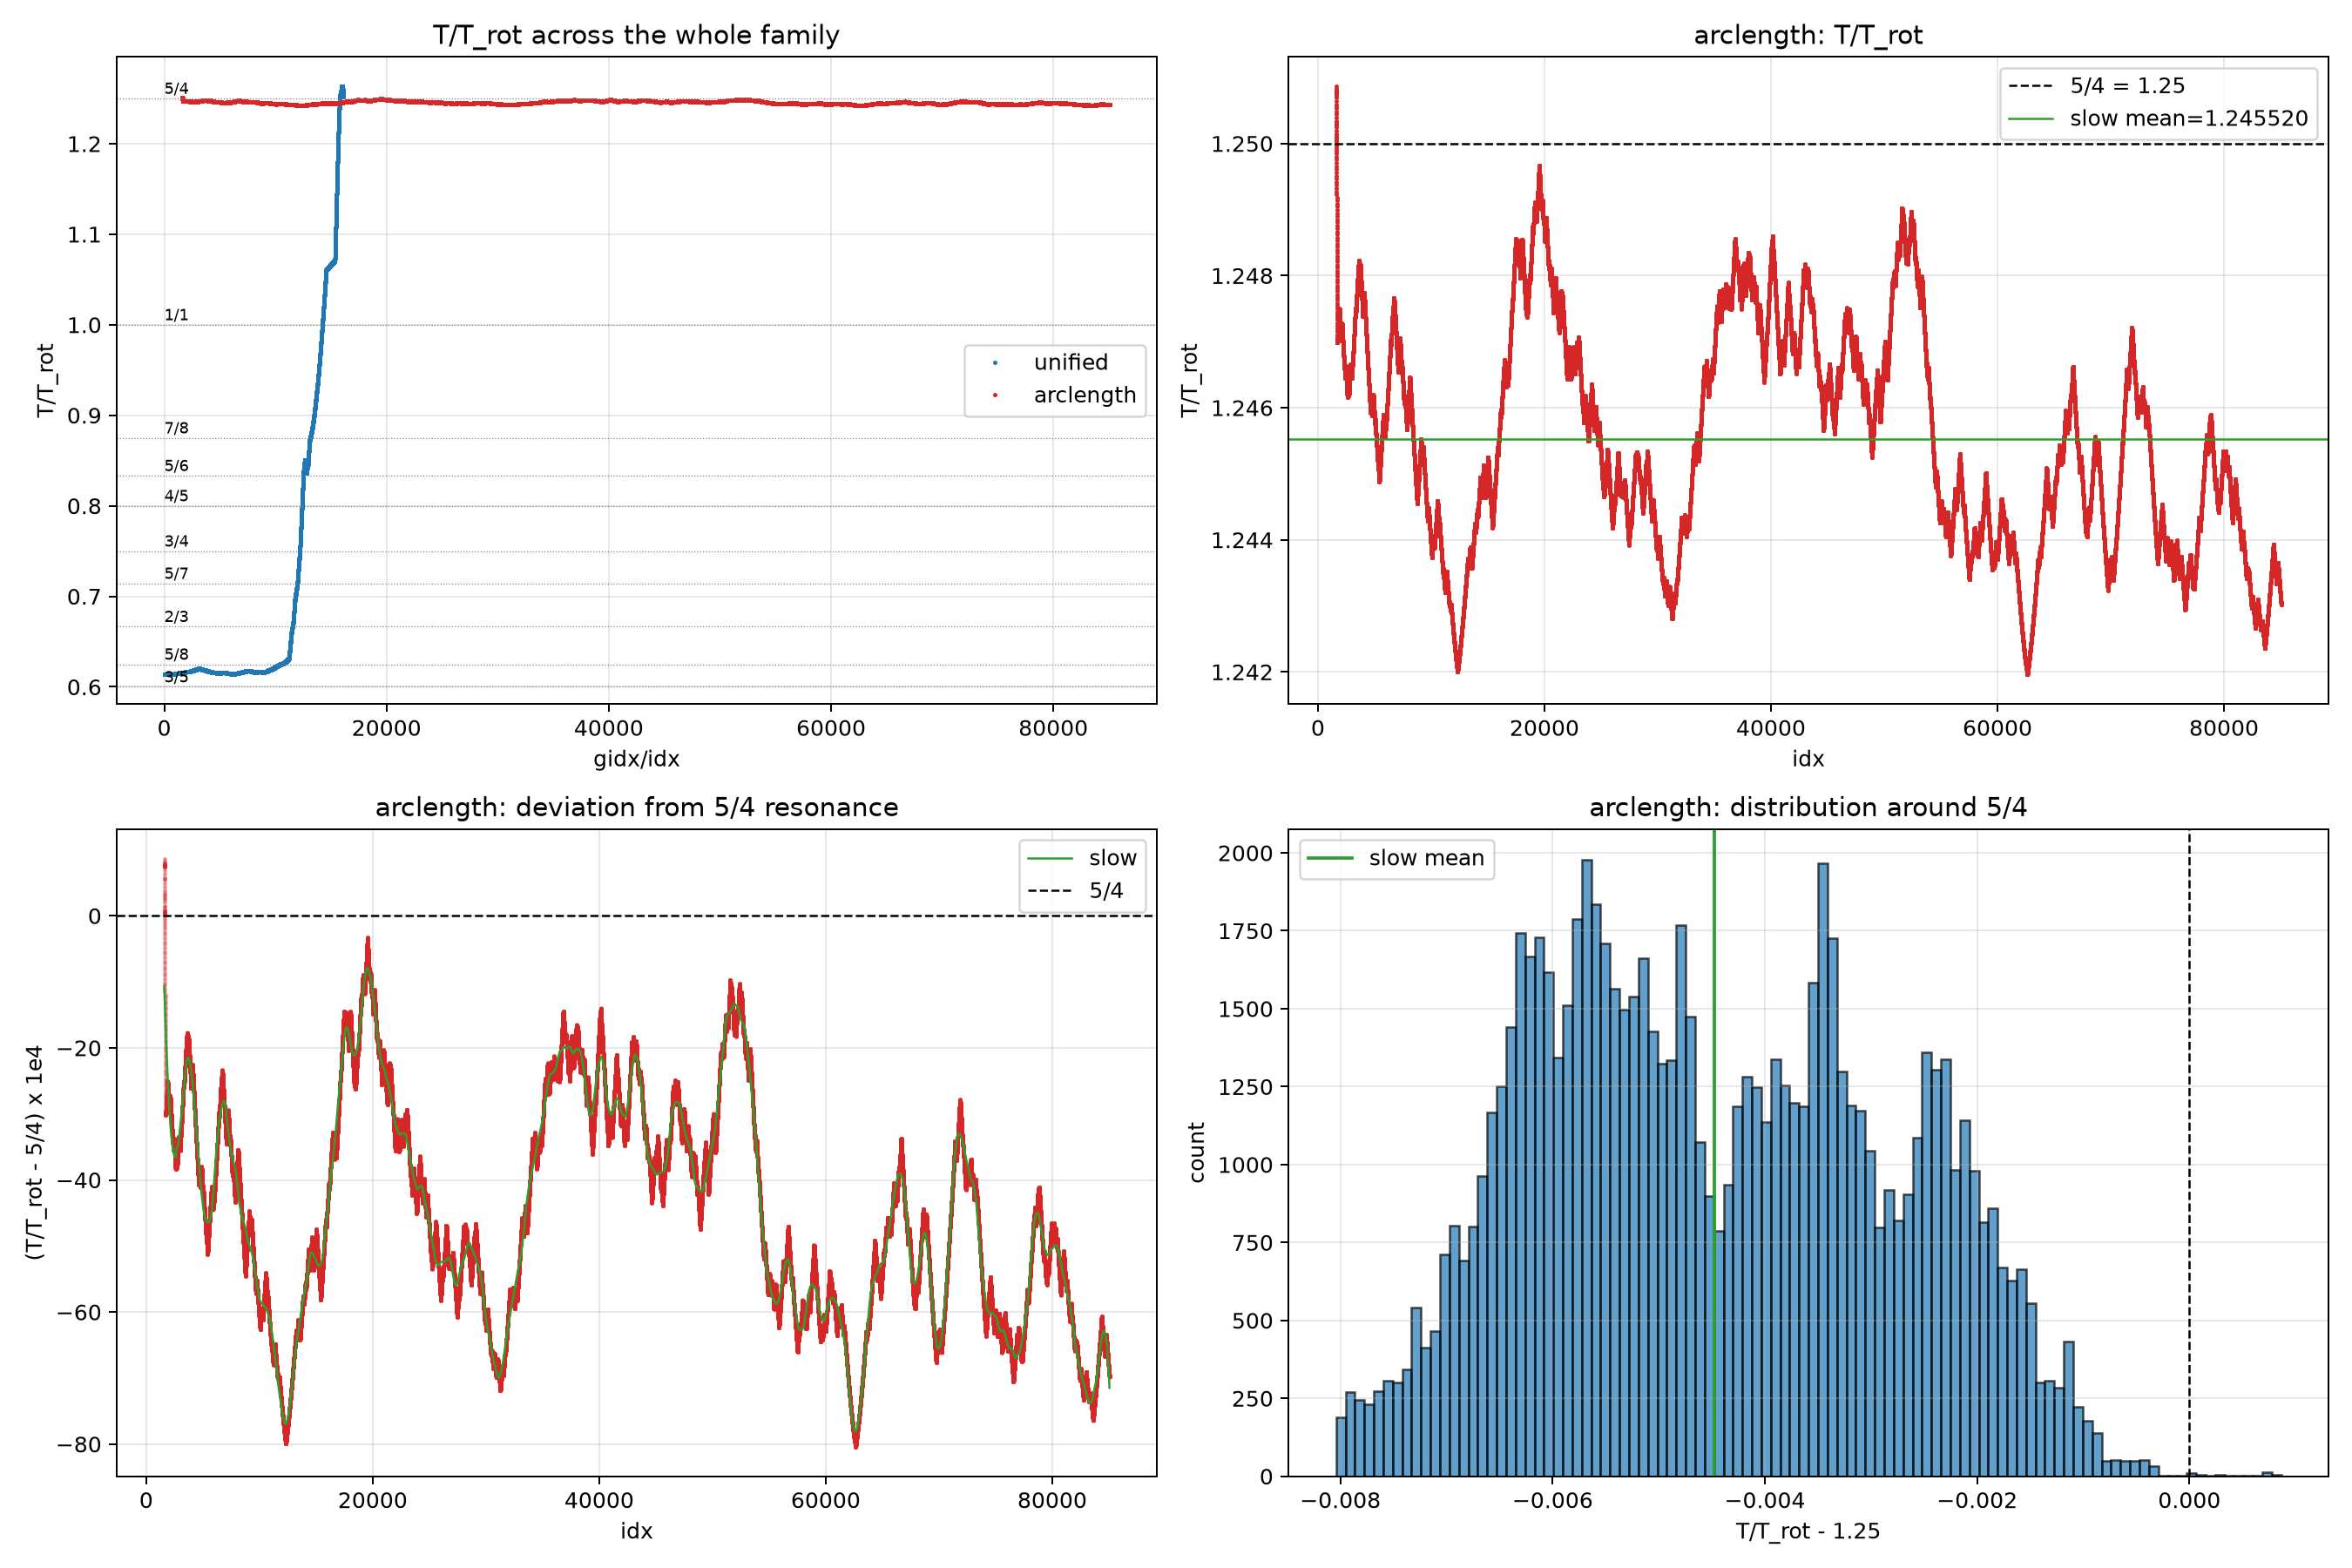
\includegraphics[width=0.75\textwidth]{49_resonance_check.png}
    \caption{Проверка гипотезы о резонансе 5/4. Зависимость периода \(T\) от \textit{mean\_dev} монотонна, «плато» в блоке arclength — следствие узости интервала, а не резонансного захвата.}
    \label{fig:resonance_check}
\end{figure}

\subsection{Широкополосность медленной моды}
Анализ автокорреляционной функции (АCF) и структурной функции орбит (рисунок~\ref{fig:acf}) показал, что так называемая «медленная мода», определяющая форму огибающей орбиты и изменение параметров вдоль семейства, не разлагается на 2–4 четко выраженные гармоники. Она представляет собой широкополосный процесс. Это указывает на сложную нелинейную природу динамики, а не на присутствие одного доминирующего квазипериодического движения.

\begin{figure}[H]
    \centering
    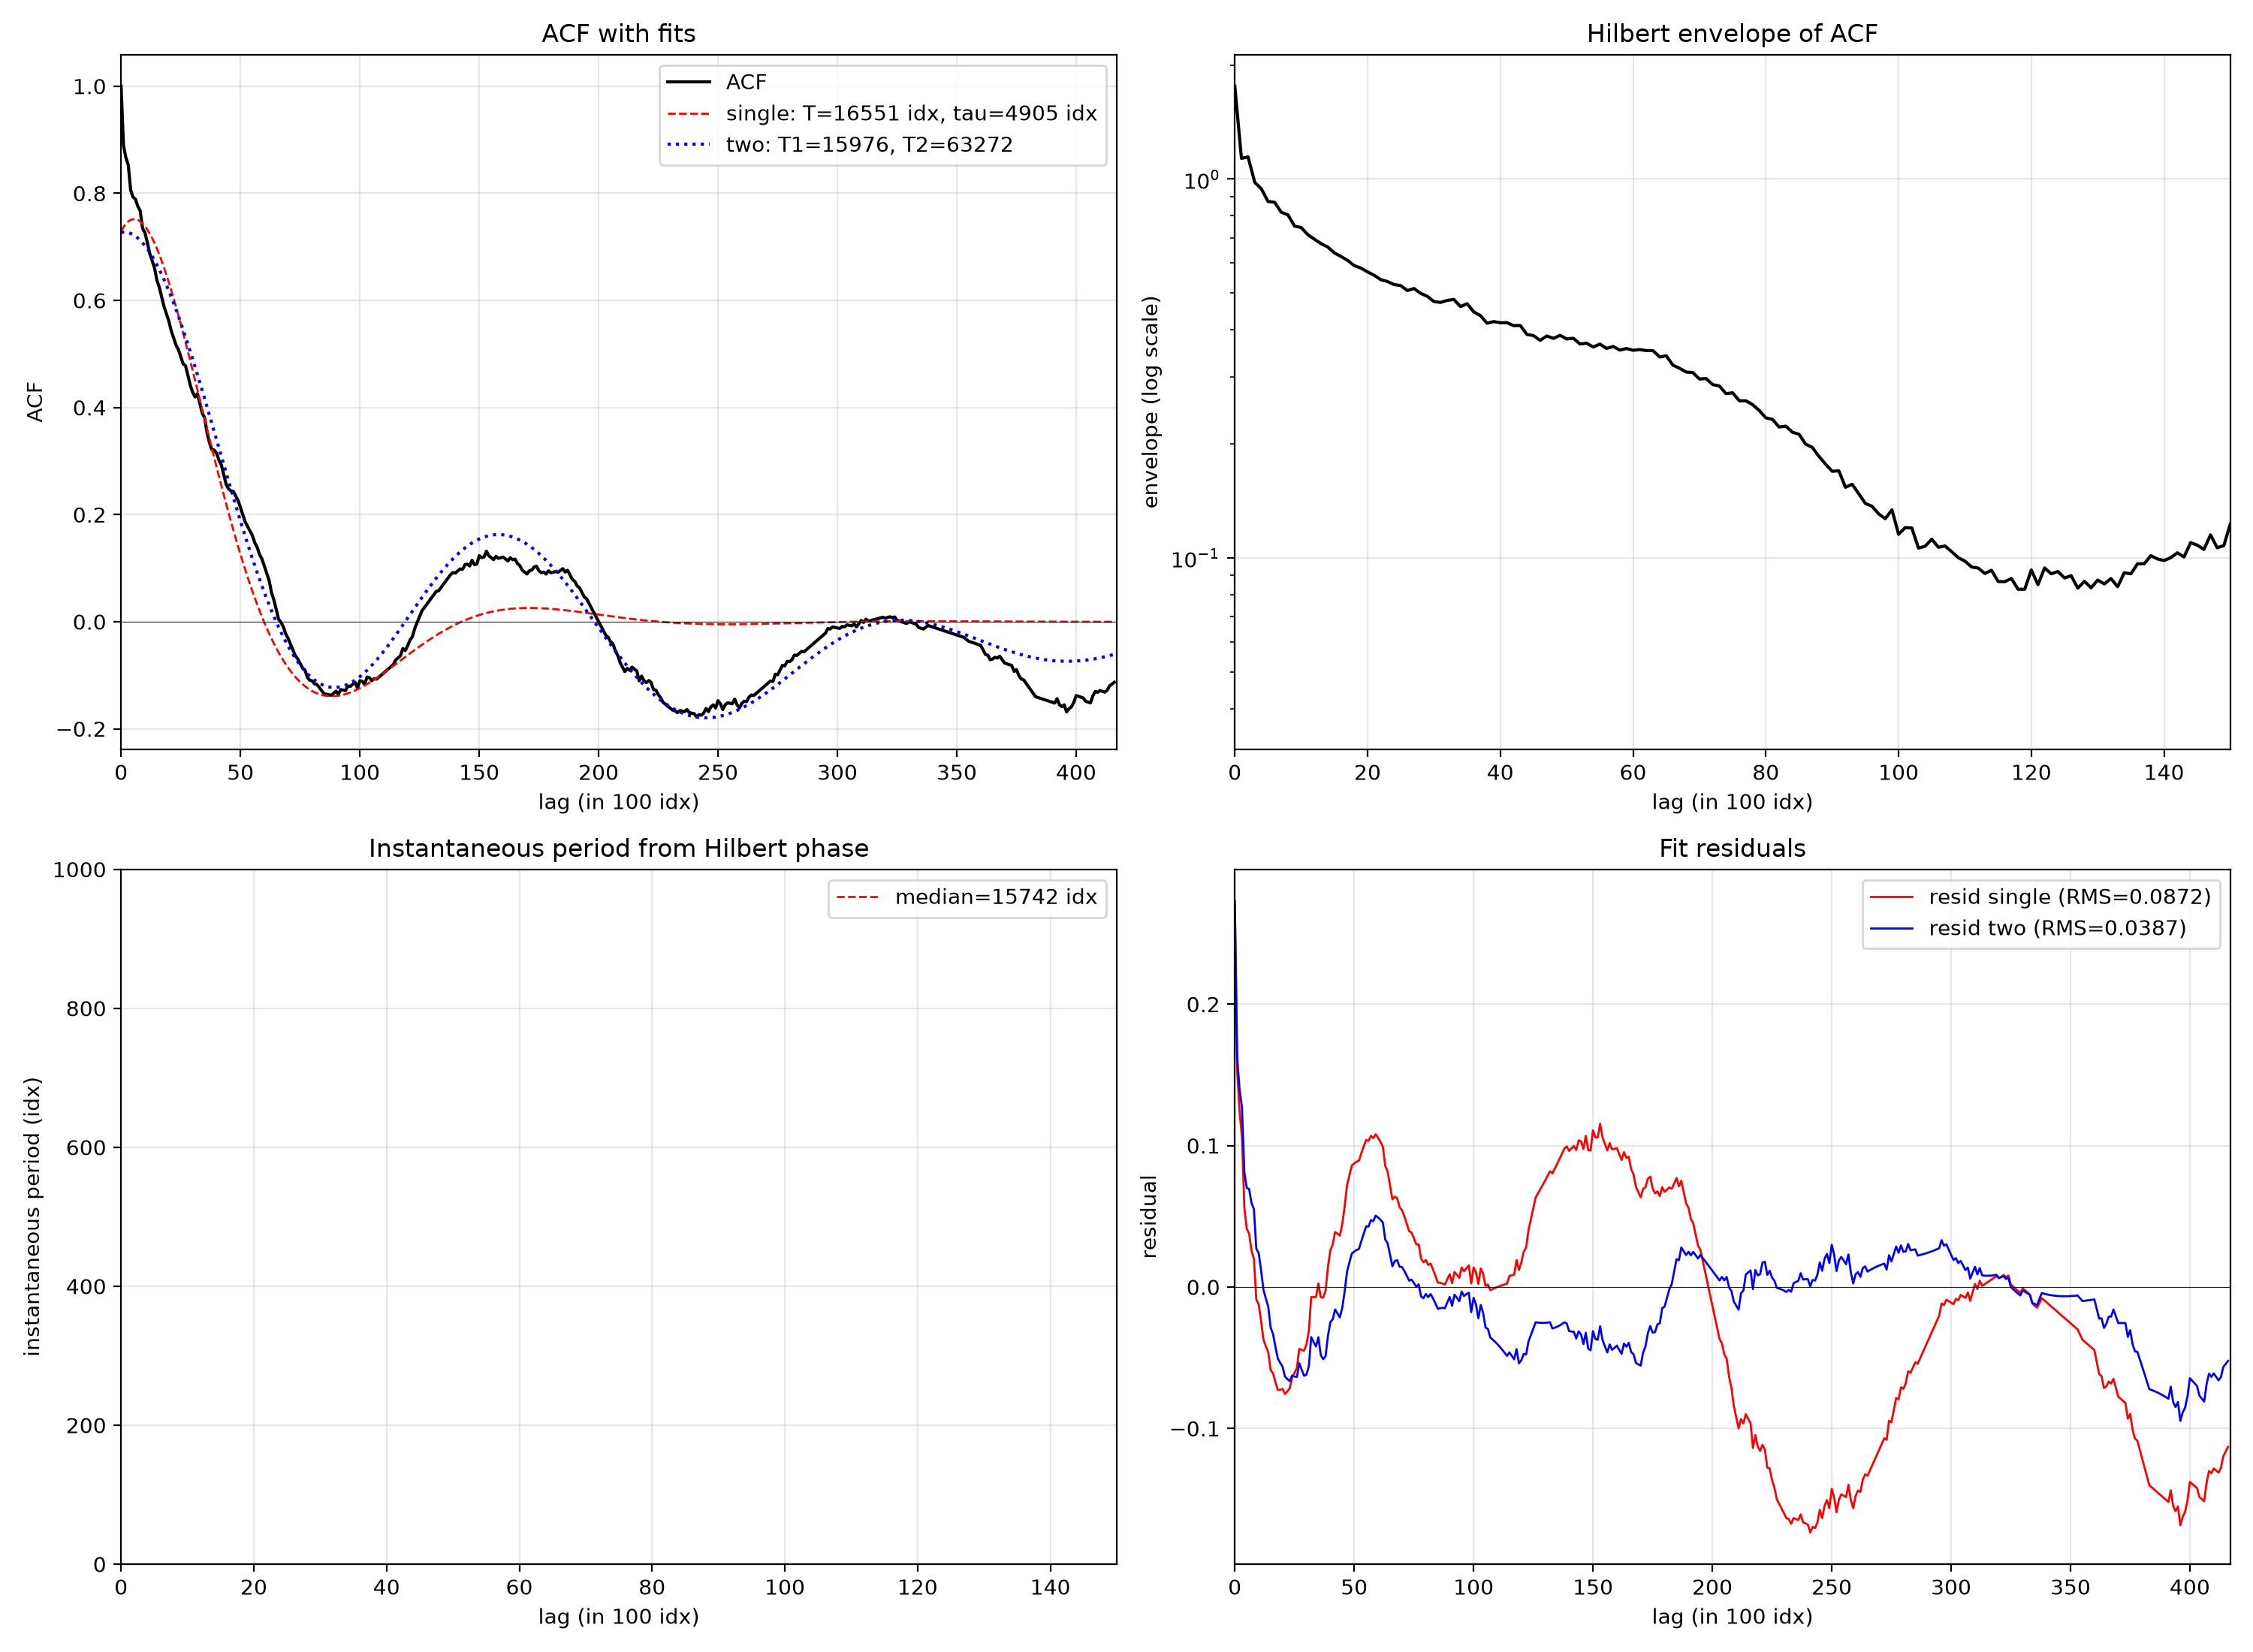
\includegraphics[width=0.75\textwidth]{69_acf_analysis.png}
    \caption{Автокорреляционная функция (ACF), демонстрирующая широкополосный характер медленной динамики вдоль семейства.}
    \label{fig:acf}
\end{figure}

% Общий мастер-плот (по желанию можно вставить здесь или в заключение)
\begin{figure}[H]
    \centering
    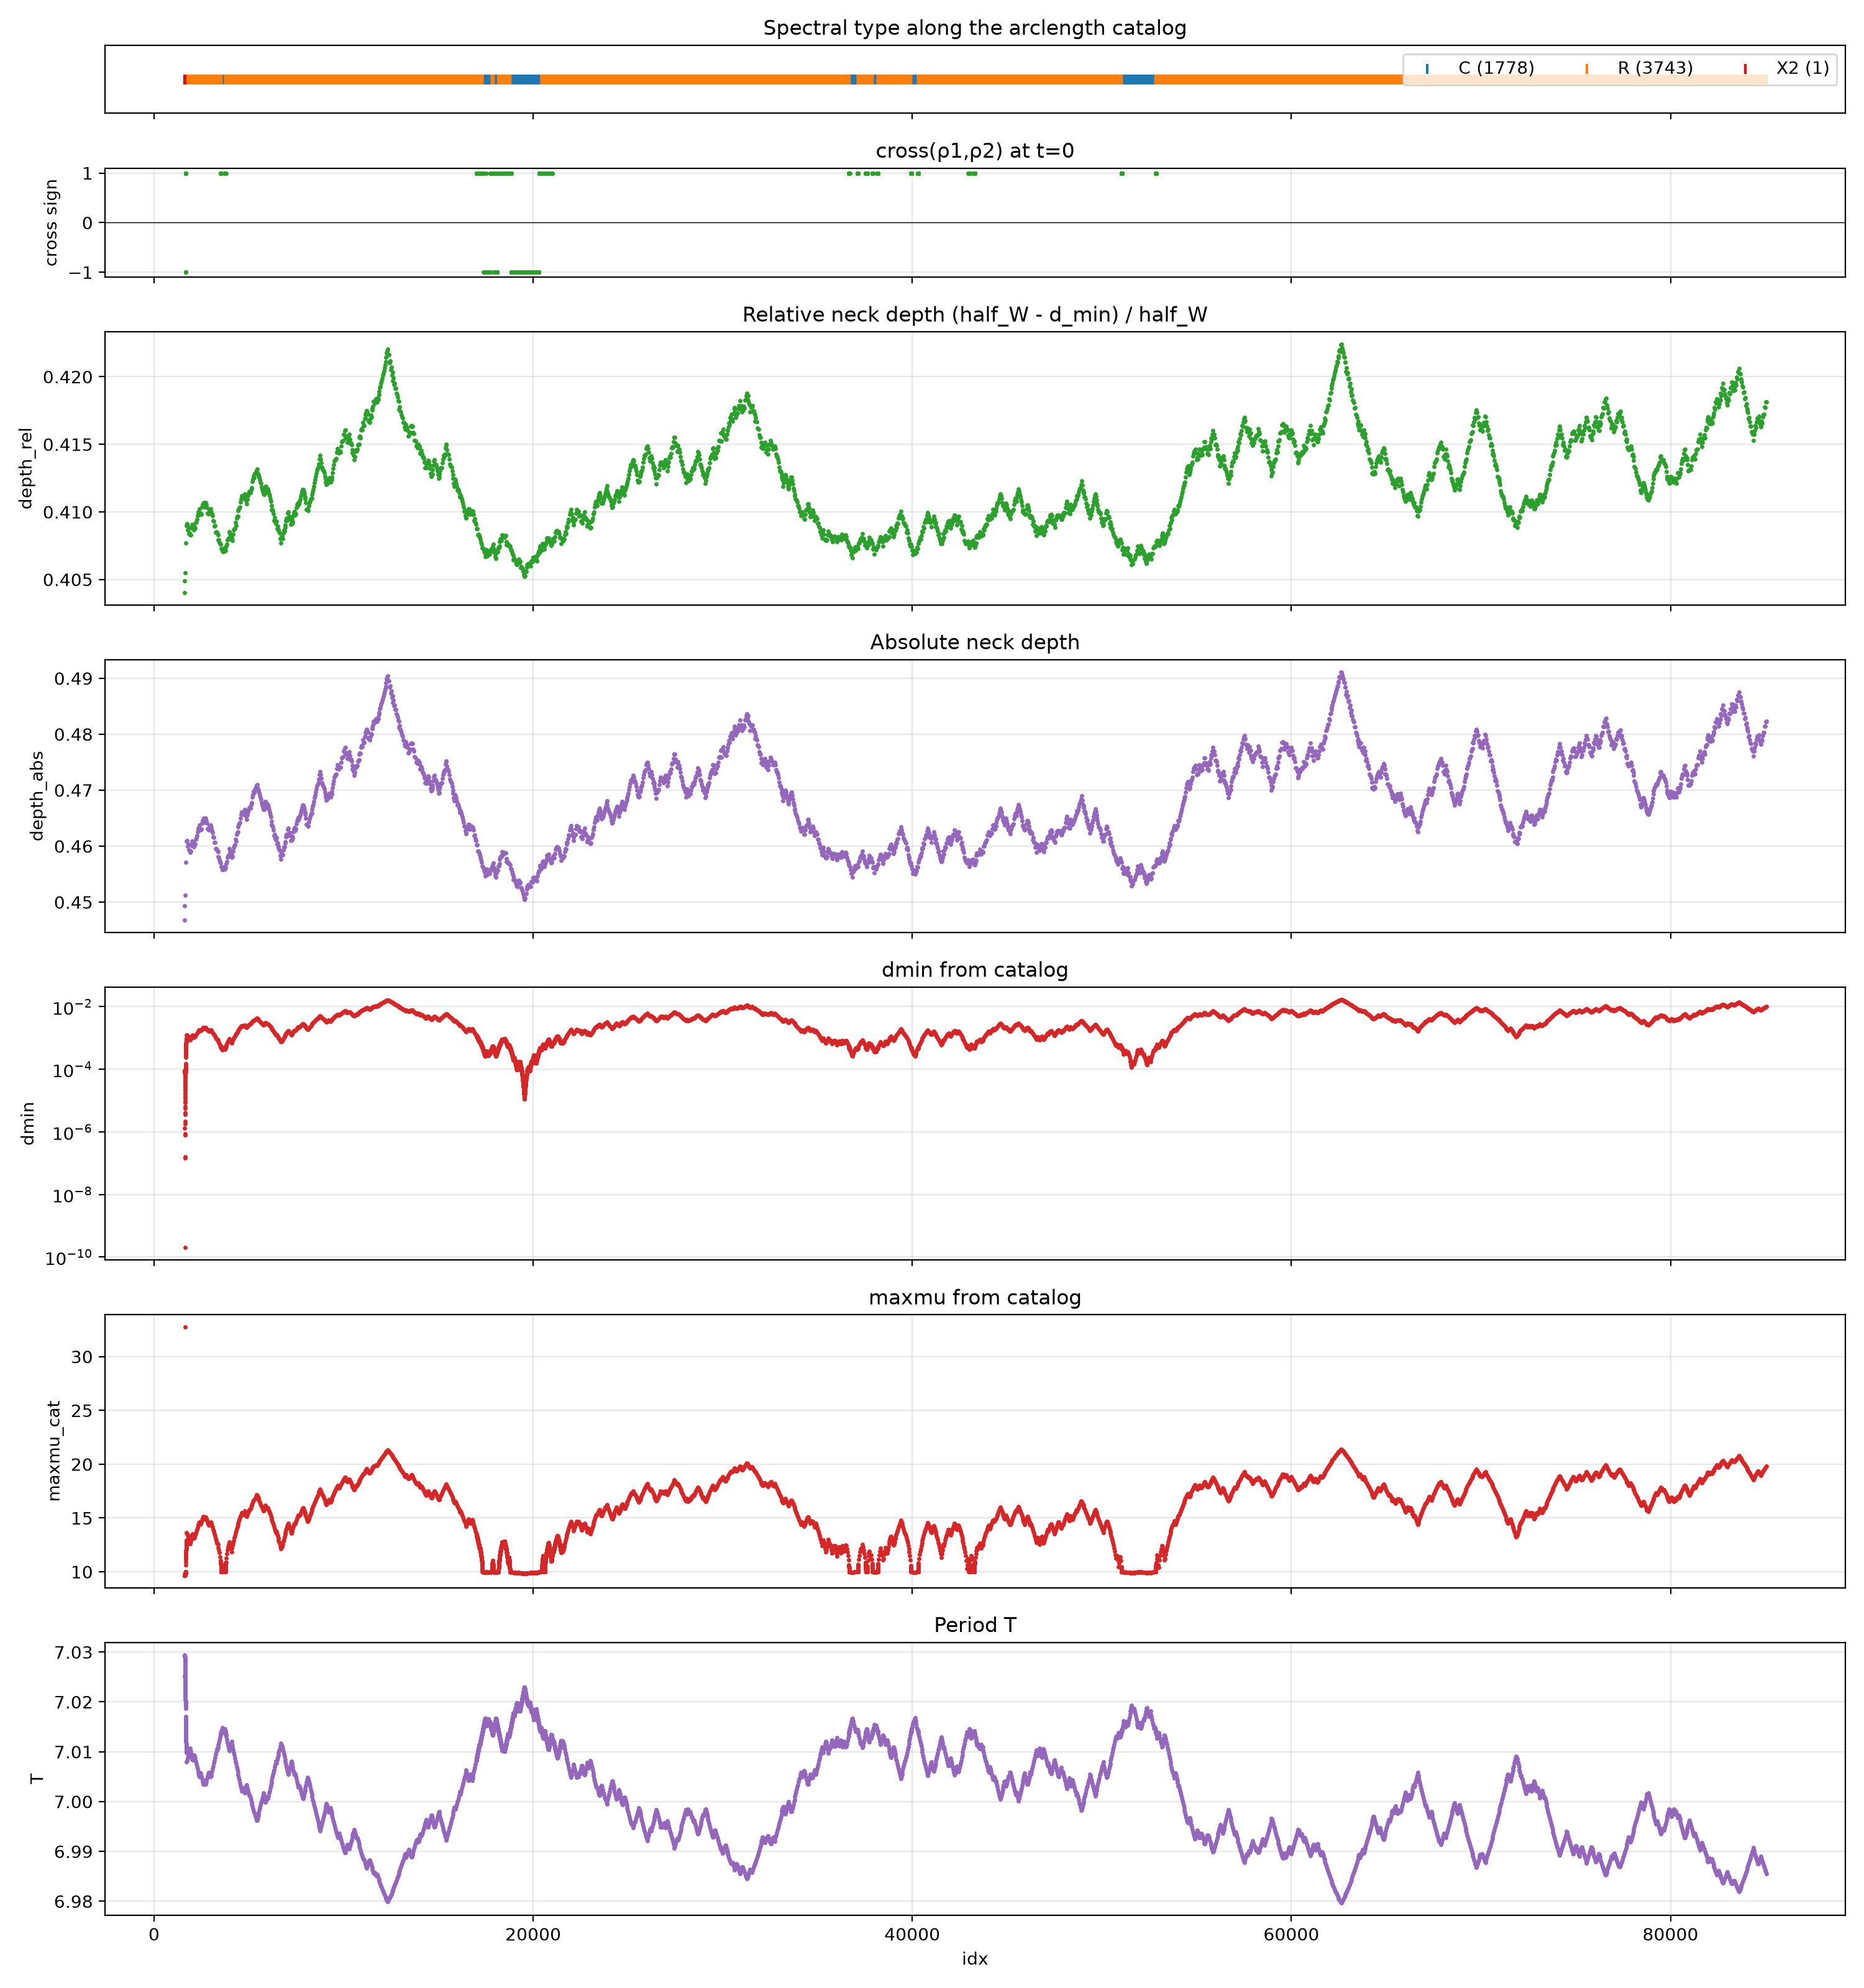
\includegraphics[width=0.95\textwidth]{27_master_plot.png}
    \caption{Общая карта семейства: \(T\), \(\lambda\), \(d_{\min}\), \(\max|\mu|\), глубина ямки и типы спектров.}
    \label{fig:master_plot}
\end{figure}

\section{Симметрии и топология относительного движения}

В этом разделе исследуются симметрии системы и орбит, структура Жордана для тривиального мультипликатора \(\mu=1\) и топология относительного движения тел (числа обхода). Эти аспекты важны для понимания того, что является физическим механизмом переходов в семействе, а что — геометрическим следствием изменения амплитуды.

\subsection{Симметрии системы и орбит}
Уравнения движения в плоской задаче трёх тел с равными массами обладают группой симметрий, порождённой перестановками тел \(\sigma_{12}, \sigma_{13}, \sigma_{23}\) и поворотом на \(\pi\) (обозначим \(R_\pi\)). Все восемь элементов группы (включая композиции \(\sigma_{ij} \cdot R_\pi\)) проверены численно: для каждой из них выполняется тождество
\begin{equation}
    S \cdot f(X) = f(S \cdot X)
\end{equation}
с точностью до машинного нуля.

Для самих периодических орбит единственной нетривиальной симметрией оказалась
\begin{equation}
    X(T/2) = (\sigma_{13} \cdot R_\pi) \cdot X(0),
\end{equation}
то есть через половину периода орбита переходит в себя при перестановке тел 1 и 3, совмещённой с поворотом на \(\pi\). Тождество выполняется с точностью \(10^{-11}\) для орбит малой амплитуды и \(10^{-3}\) для орбит с большими амплитудами (что соответствует накопленной ошибке интегрирования на длинных периодах). Остальные элементы группы дают расстояние \(\sim |X_0|\), то есть не являются симметриями орбит.

\subsection{Структура Жордана для \(\mu=1\)}
Для тривиального мультипликатора \(\mu=1\) во всём семействе (кроме начальной точки \(gidx=0\), лежащей на самом равновесии) структура Жордана имеет вид
\begin{equation}
    J_2 + J_2,
\end{equation}
то есть матрица монодромии имеет две жордановы клетки размера 2. Это \textbf{стандартная} структура для однопараметрического семейства периодических орбит в гамильтоновой системе: две жордановы клетки отвечают сдвигу вдоль орбиты и сдвигу вдоль семейства. Скрытой симметрии, порождающей дополнительную кратность (как \(J_3\) или \(J_4\)), в семействе нет.

\subsection{Числа обхода: тела вокруг своих равновесий}
Были вычислены числа обхода траекторий каждого тела вокруг своей точки равновесия (тела 1 и 3 — вокруг \((\pm 1, 0)\), тело 2 — вокруг \((0,0)\)), а также числа обхода величин \(\rho_1\) и \(\rho_2\) вокруг точек столкновений. Результат:
\begin{itemize}
    \item число обхода каждого тела вокруг своего равновесия \textbf{всегда равно} \(w = -1\) для всех орбит семейства;
    \item число обхода \(\rho_2\) вокруг точки столкновения 1–2 всегда равно \(0\);
    \item число обхода \(\rho_1\) вокруг точки столкновения равно \(0\) в блоке \textit{unified} до \(gidx \approx 16111\), затем равно \(-1\); в блоке \textit{arclength} оно равно \(-1\) или \(-2\) с 45 переходами.
\end{itemize}
Полная симметрия тел 1, 2, 3 вокруг своих равновесий (\(w=-1\) у всех) подтверждает симметрию равных масс и является геометрическим свойством орбит Ляпунова.

\subsection{Интерпретация переходов числа обхода \(\rho_1\): \(0 \to -1\)}
Изменение числа обхода \(\rho_1\) вокруг точки столкновения с \(0\) на \(-1\) при \(gidx \approx 16111\) не является топологической бифуркацией в смысле смены класса орбиты. Это \textbf{геометрическое следствие роста амплитуды}: при увеличении амплитуды траектория \(\rho_1(t)\) начинает охватывать точку столкновения, и число обхода меняется скачком.

Порог по относительной глубине ямки для этого события составляет \(0.4110\), в то время как порог для переходов C \(\leftrightarrow\) R составляет \(0.4076\). Оба порога близки и соответствуют геометрическому условию «орбита начинает охватывать точку», а не какому-либо динамическому механизму.

\subsection{Связь числа обхода с устойчивостью}
Прямой связи между числами обхода и переходами C \(\leftrightarrow\) R не обнаружено: медианное расстояние между событиями составляет \(\sim 2300\) индексов, ни одного точного совпадения нет. Аналогично, корреляция \(\lambda\) с числом обхода после удаления влияния \(T\) оказывается слабой. В плоскости \((\text{depth}, \lambda)\) точки с \(w=-1\) и \(w=-2\) ложатся на одну и ту же кривую, то есть число обхода не является независимым параметром, а определяется амплитудой (глубиной ямы).

\begin{figure}[H]
    \centering
    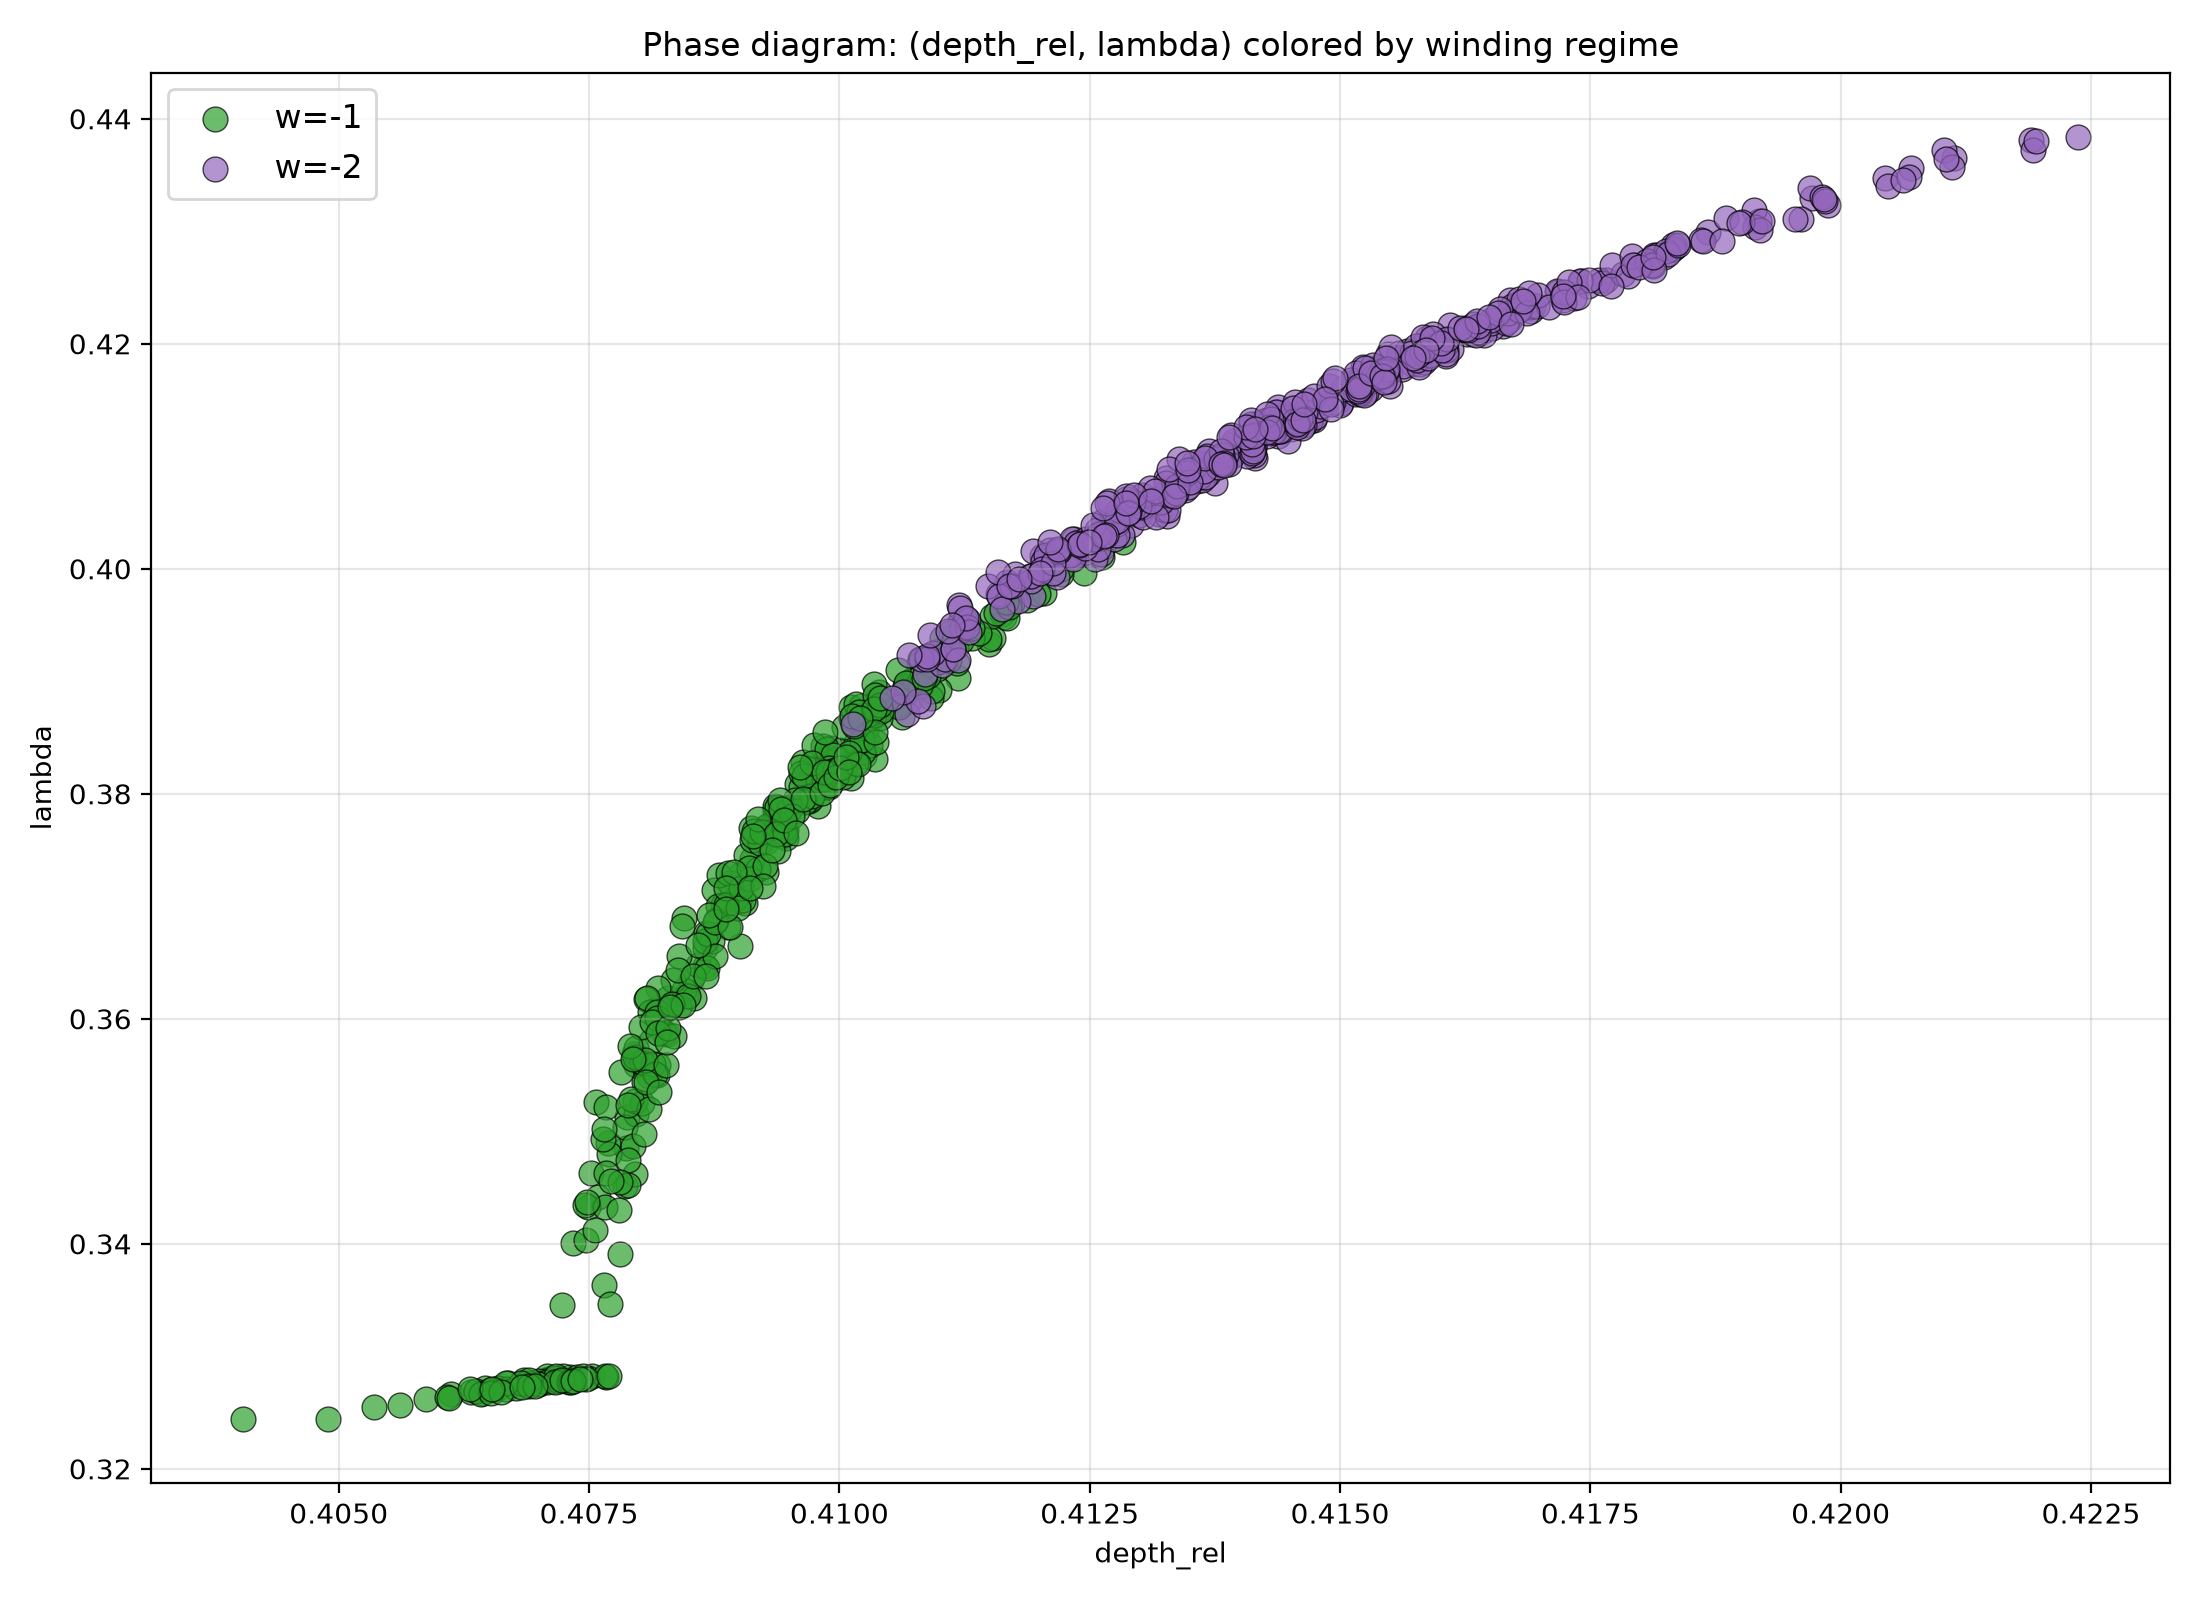
\includegraphics[width=0.8\textwidth]{67_phase_diagram.png}
    \caption{Фазовая диаграмма в плоскости \((\text{depth}, \lambda)\). Точки с разными числами обхода лежат на одной кривой, что указывает на отсутствие независимой связи между числом обхода и устойчивостью.}
    \label{fig:phase_diagram_winding}
\end{figure}

\begin{figure}[H]
    \centering
    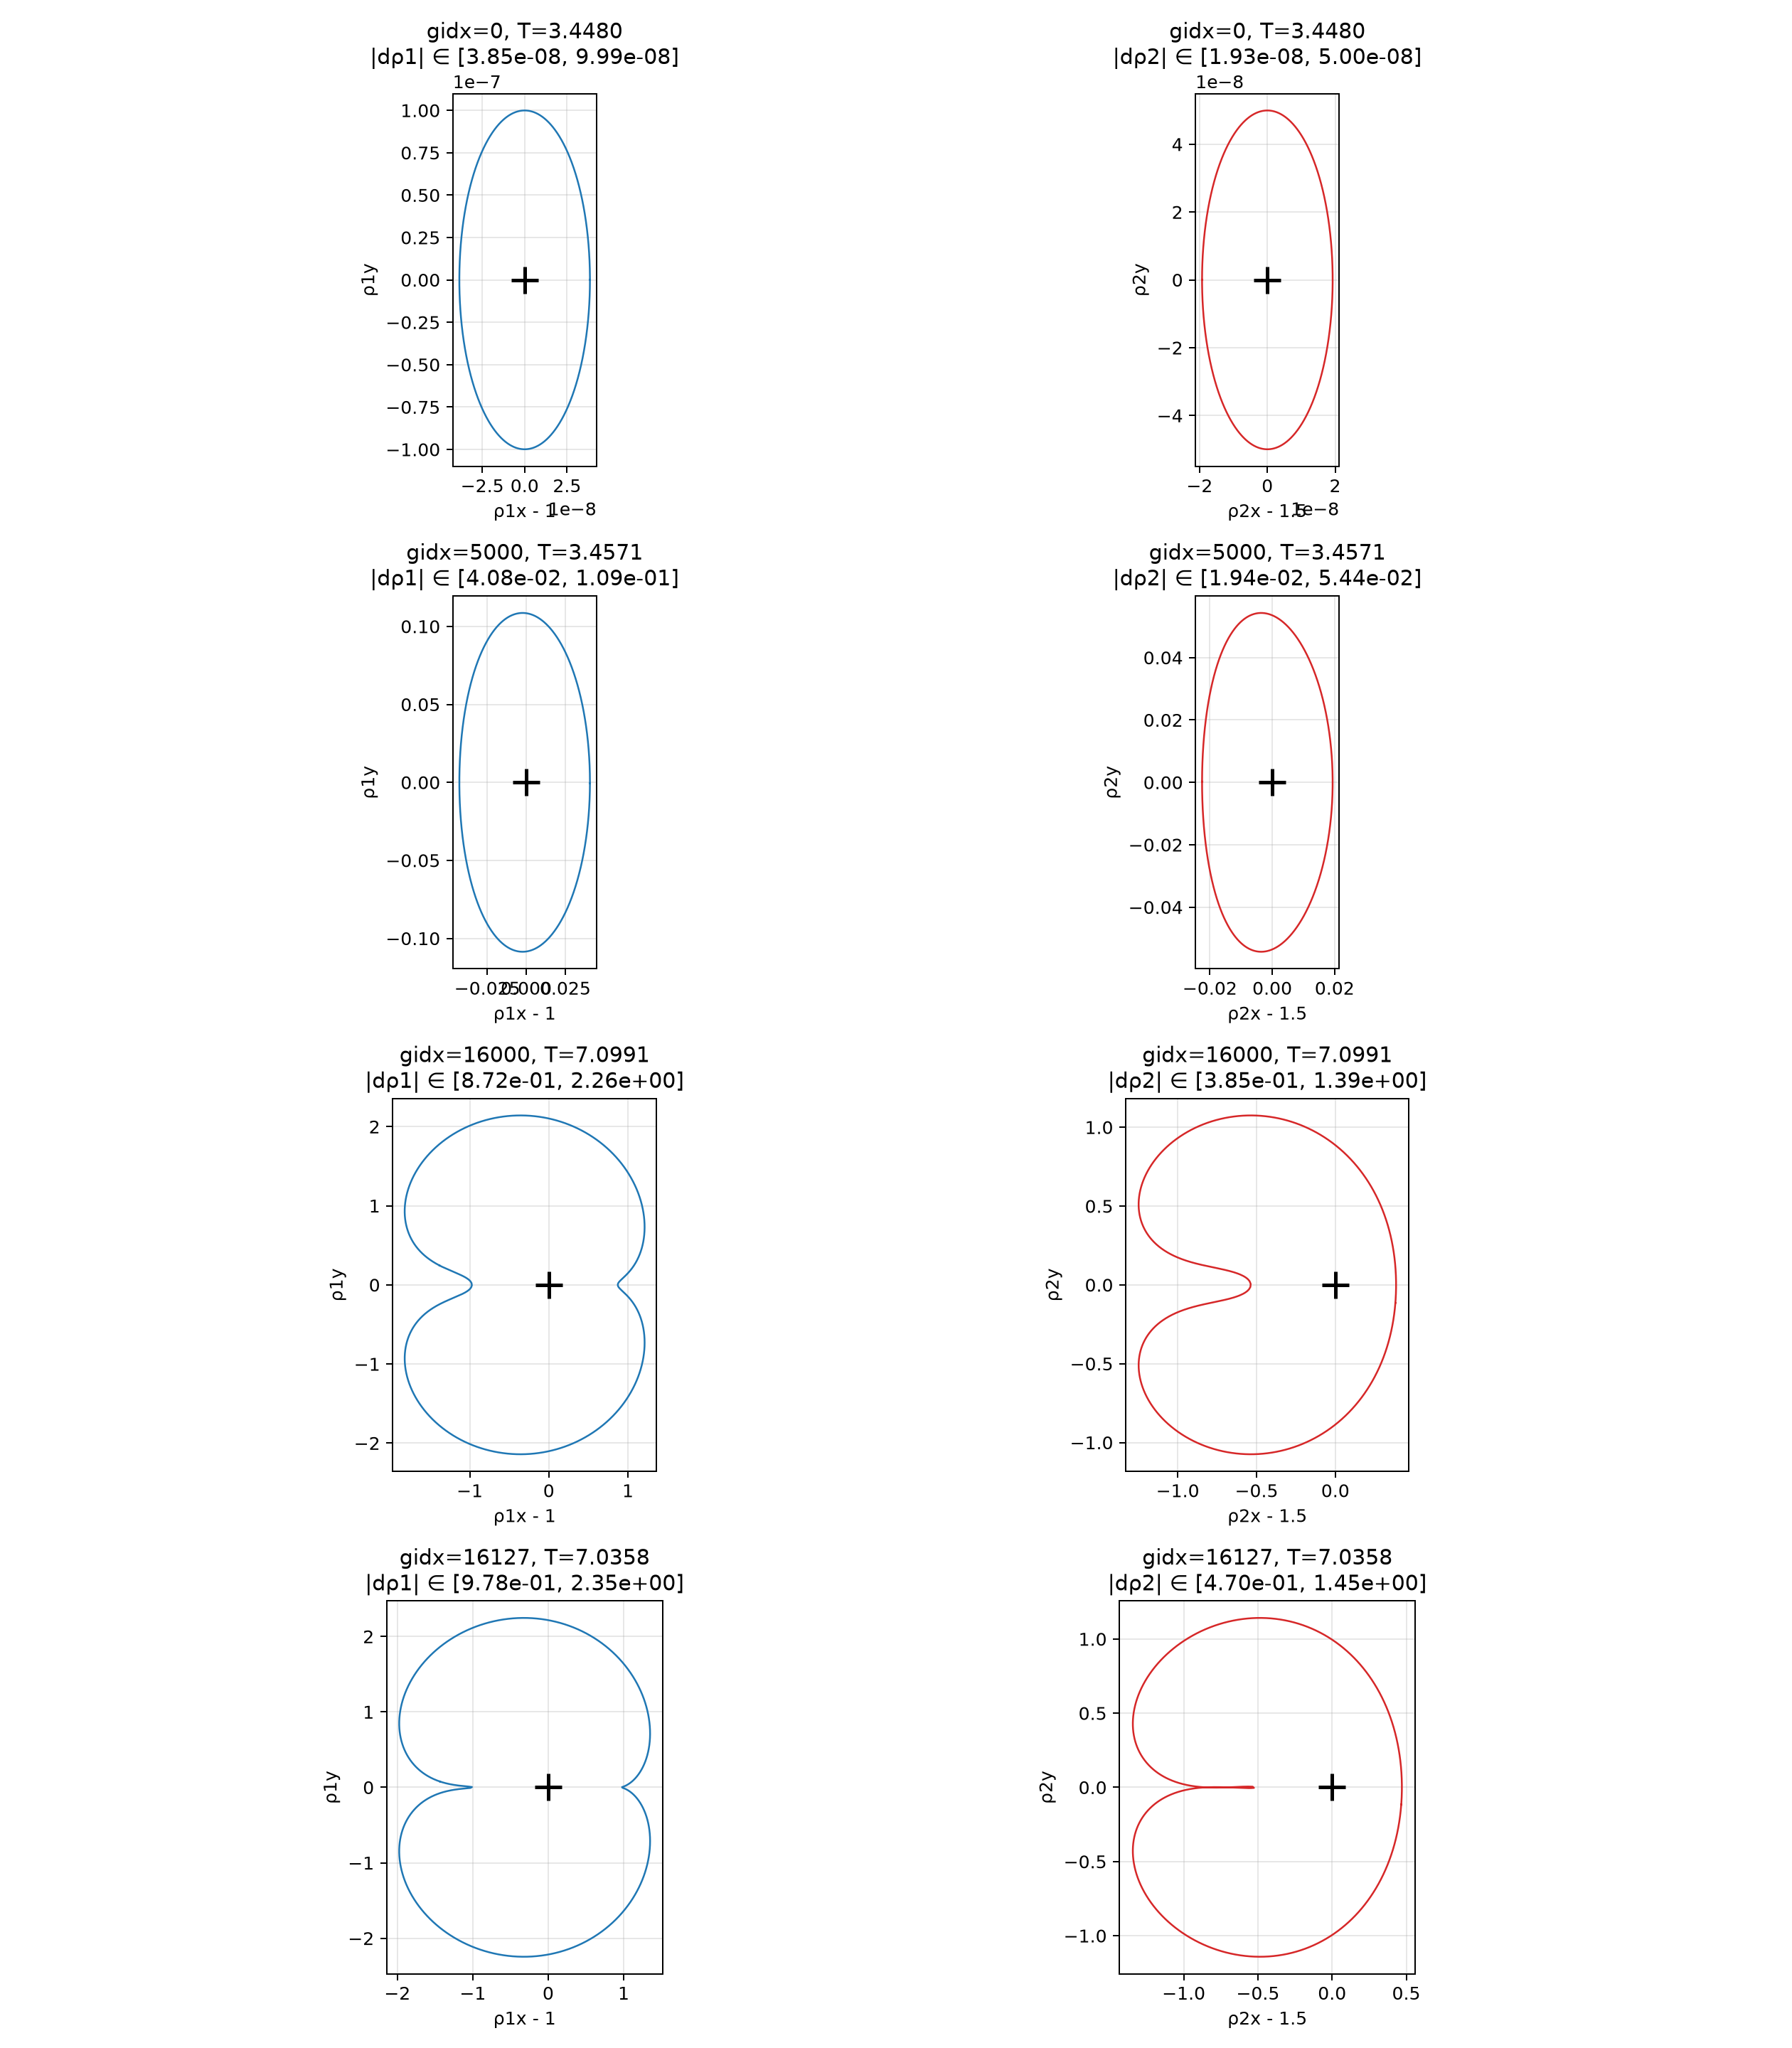
\includegraphics[width=0.85\textwidth]{88_libration_anatomy.png}
    \caption{Анатомия либрации: эллипс вокруг равновесия и восьмёрка. Число обхода каждого тела вокруг своего равновесия \(w=-1\) — следствие полного обхода за период.}
    \label{fig:libration_anatomy}
\end{figure}

\section{Глубокие сближения, поверхность нулевой скорости и \(\xi\)-пространство}

Одной из ключевых задач исследования было понять, что происходит с орбитами при экстремально глубоких сближениях тел, и связаны ли эти сближения с какими-либо бифуркациями или с касанием границы области допустимого движения (поверхности нулевой скорости). В этом разделе показано, что наблюдаемые аномалии в спектре при \(d_{\min} \sim 10^{-10}\) являются артефактом точности, а не физикой, а поверхность нулевой скорости нигде не достигается.

\subsection{Разбор орбиты 1641: артефакт точности real128}
В блоке \textit{arclength} была найдена орбита с индексом \(idx=1641\), у которой минимальное расстояние между телами достигает \(d_{\min} = 1.97 \times 10^{-10}\), что на 5–8 порядков меньше, чем у остальных орбит семейства. При интегрировании в стандартной точности \texttt{real128} (\(\text{tol}=10^{-25}\)) для этой орбиты наблюдался спектр типа X2 (с двумя парами мультипликаторов, близких к \(+1\)) и аномально большое значение \(\max|\mu| = 32.7\), резко выделяющееся на фоне соседних орбит (\(\max|\mu| \approx 9.78\)).

Для выяснения природы этой аномалии были проведены систематические тесты:
\begin{enumerate}
    \item Переинтегрирование с точностью 64, 128, 192, 256 и 384 бита. Значение \(d_{\min}\) воспроизводится с точностью \(0.03\%\) на всех уровнях точности, то есть сближение реально.
    \item При \(\text{prec}=256\) (\(\text{tol}=10^{-60}\)) спектр меняется: вместо X2 наблюдается тип C с \(\max|\mu| = 9.78\), совпадающий с соседними орбитами 1640 и 1642.
    \item При \(\text{prec} \geq 256\) спектр воспроизводим и не зависит от \(\text{tol}\). При \(\text{real128}\) спектр оказался чувствительным к \(\text{tol}\) (значения 9.39, 48.8, 9.78 при \(\text{tol}=10^{-20}, \dots, 10^{-33}\)).
    \item Уточнение методом Ньютона сдвигает начальное состояние на \(\sim 10^{-12}\), а \(d_{\min}\) не меняется.
    \item Соседние орбиты 1640, 1642, 1620 при любых ограничениях метода Ньютона дают один и тот же \(d_{\min}\) и спектр.
\end{enumerate}
Вывод: \textbf{орбита 1641 не является бифуркацией}, а представляет собой артефакт точности \texttt{real128} при \(d_{\min} \sim 10^{-10}\). При повышении точности до 256 бит она ведёт себя как обычная орбита типа C. Геометрия 1641 — изоскелесная конфигурация с двумя одновременными сближениями пар (12 и 23 при \(t \approx 3.4105\); 12 и 13 при \(t \approx 6.9228\)).

\subsection{Геометрия \(\xi\)-пространства}
Для визуализации относительного движения и анализа поверхности нулевой скорости используется координатное пространство \(\xi = (\xi_1, \xi_2, \xi_3)\), введённое в разделе 2. В этих координатах:
\begin{itemize}
    \item точка равновесия \(\xi_{eq} = (-1, \sqrt{3}, 0)\);
    \item момент инерции \(I = |\xi|\);
    \item лучи коллизий (сближений пар тел 1–2, 2–3, 3–1) лежат в плоскости \((\xi_1, \xi_2)\) под углами \(\pi\), \(\pi/3\), \(-\pi/3\).
\end{itemize}
Траектории орбит в \(\xi\)-пространстве представляют собой замкнутые петли, проходящие вблизи \(\xi_{eq}\). 3D-визуализация траекторий (для нескольких репрезентативных орбит) показана на рисунке~\ref{fig:xi_space_3d}.

\begin{figure}[H]
    \centering
    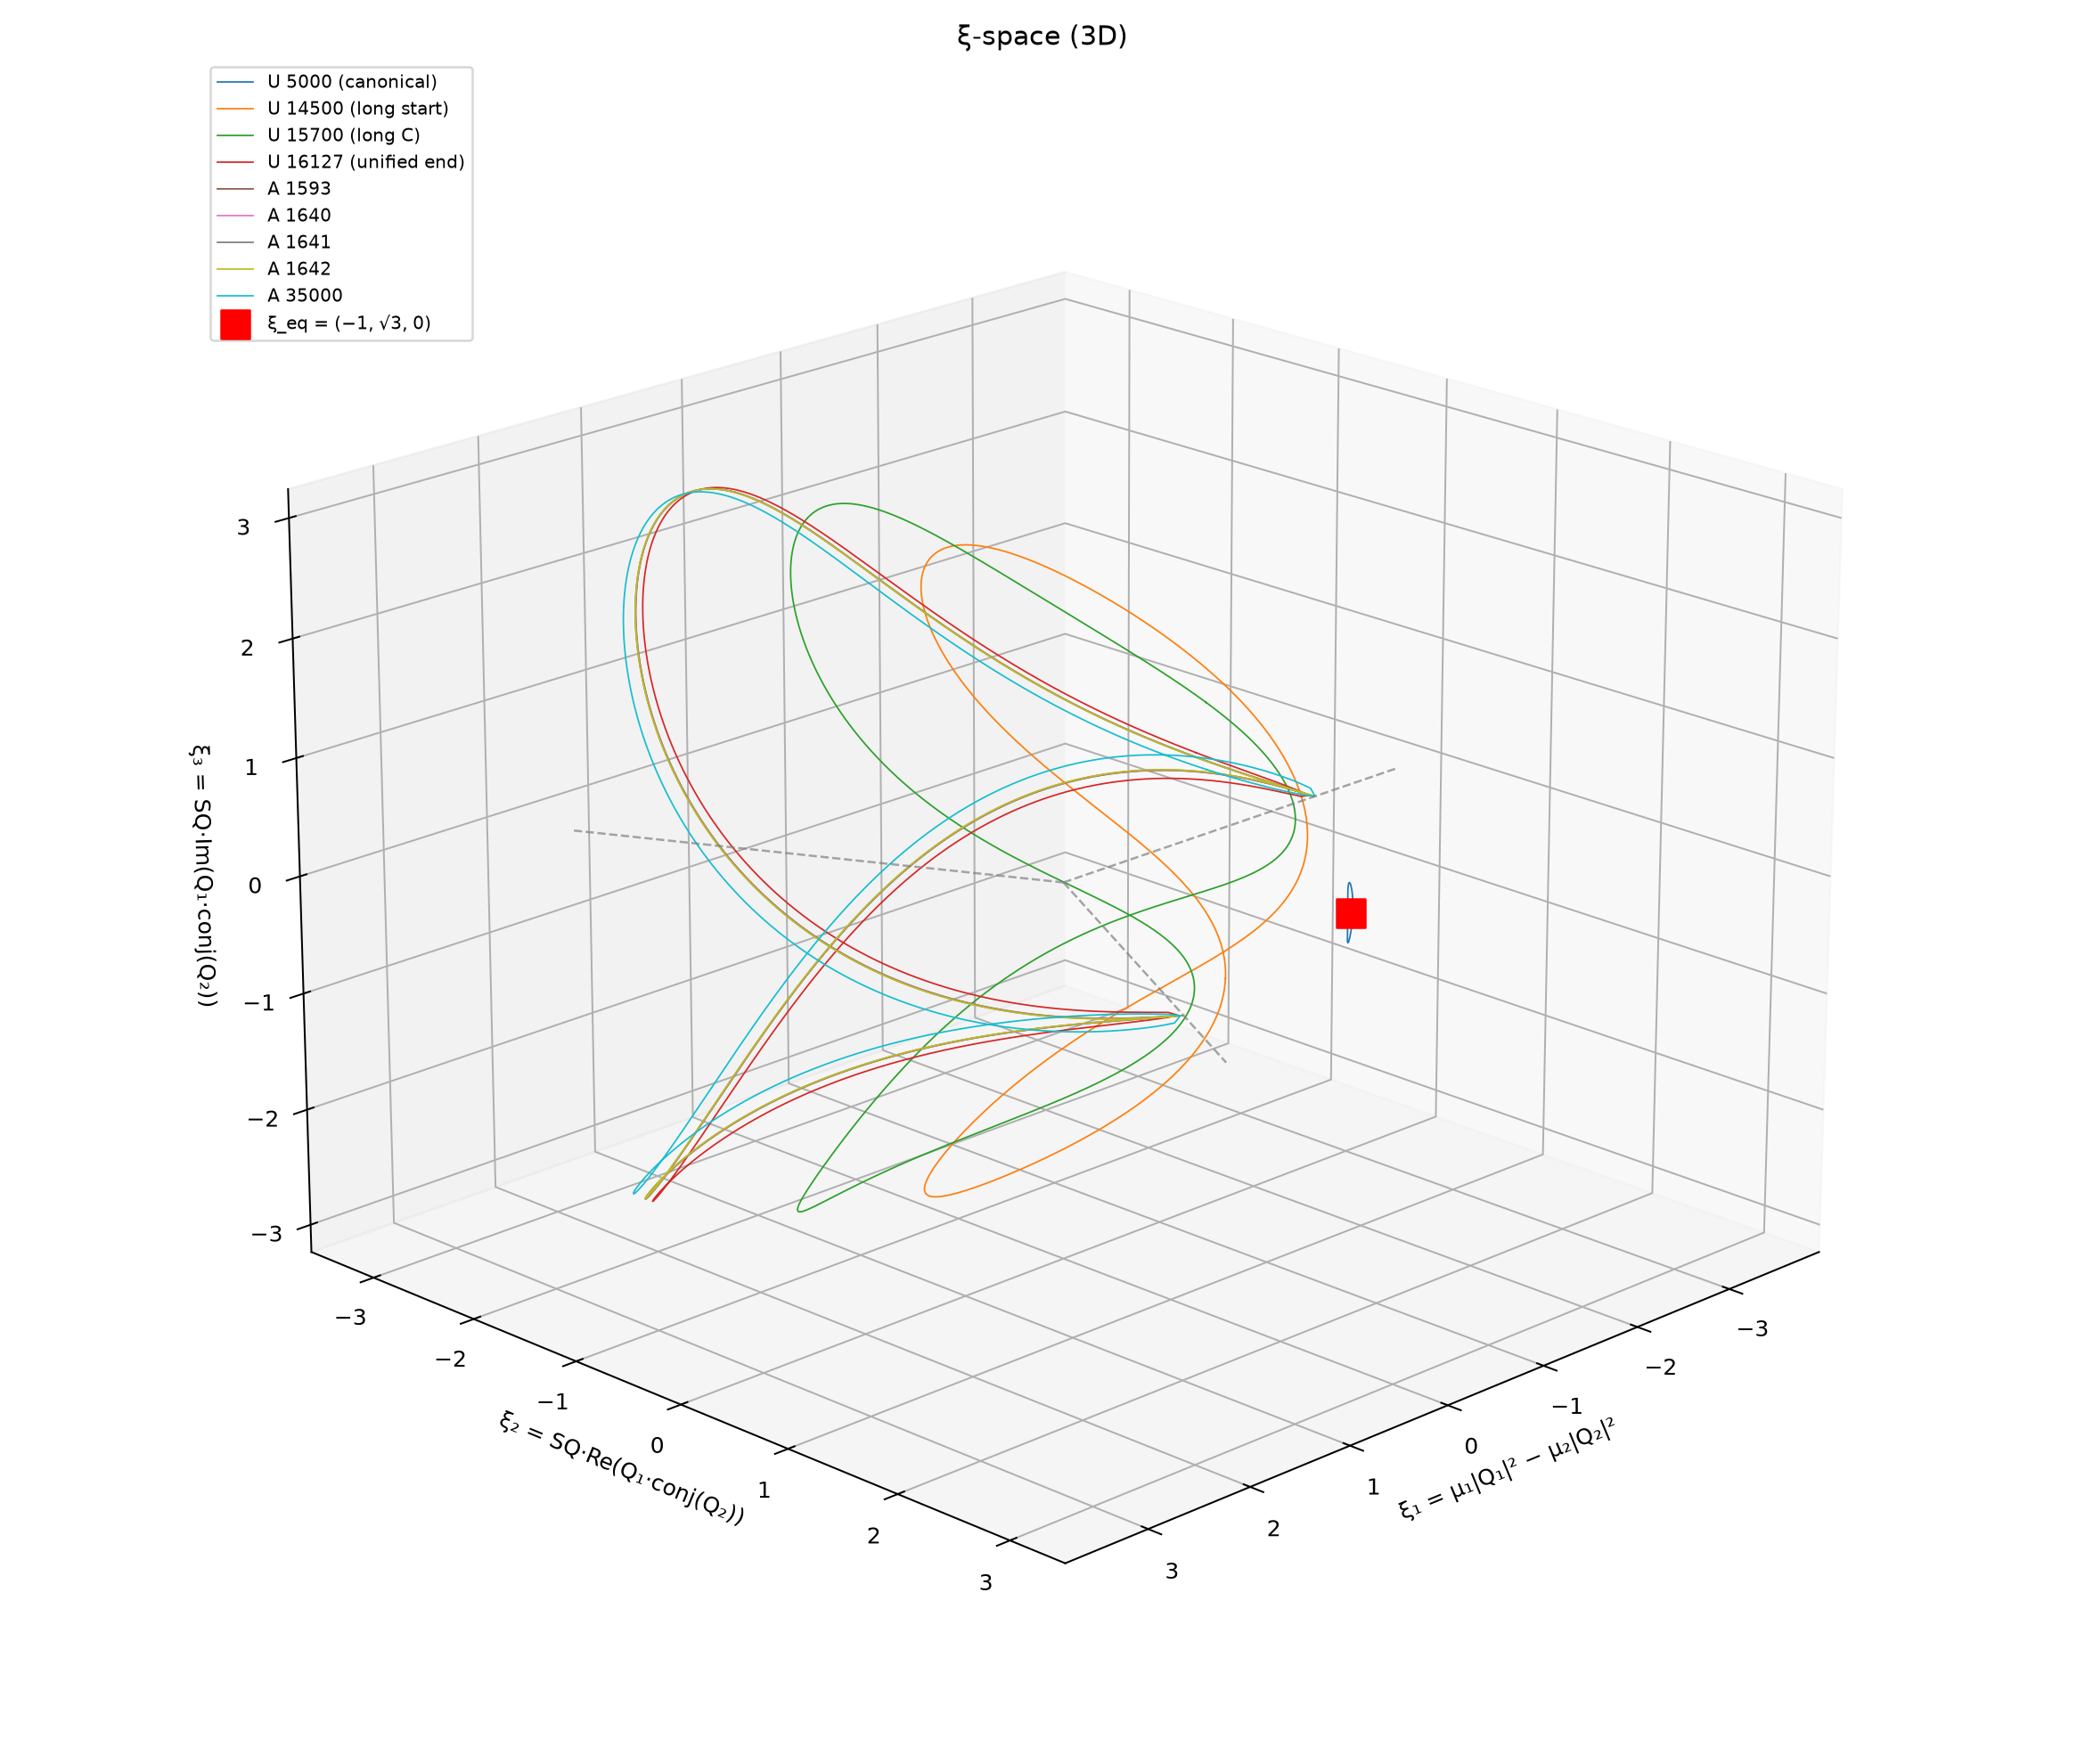
\includegraphics[width=0.85\textwidth]{93_xi_space_3d_v3.png}
    \caption{Траектории орбит в \(\xi\)-пространстве (3D). Точка \(\xi_{eq} = (-1, \sqrt{3}, 0)\) отмечена красным квадратом.}
    \label{fig:xi_space_3d}
\end{figure}

\subsection{Поверхность нулевой скорости в \(\xi\)-пространстве}
Поверхность нулевой скорости (ZVS) задаётся уравнением Сундмана (см. раздел 2):
\begin{equation}
    V(\xi) + \frac{L_z^2}{2|\xi|} = h_{in},
\end{equation}
где \(V(\xi)\) — потенциал, \(L_z\) — полный момент импульса в инерциальной системе, \(h_{in}\) — полная энергия в инерциальной системе. Область, где левая часть меньше \(h_{in}\), является доступной для движения; за её пределами движение невозможно.

Для всех орбит семейства \(h_{in} < 0\) (от \(-1.25\) в начале до \(-1.14\) в блоке \textit{arclength}), и \(h_{in}\) никогда не проходит через ноль. Это означает, что потенциал \(V(\xi)\) компенсируется центробежным членом \(L_z^2/(2|\xi|)\), и орбиты находятся в потенциальной яме, не касаясь границы.

На рисунке~\ref{fig:zvs_2d} показаны сечения ZVS в плоскости \(\xi_3 = 0\) для трёх репрезентативных орбит (A 1593, A 1641, U 16127). Чёрная линия — граница ZVS; зелёная область — доступная для движения; синяя линия — траектория. Видно, что \textbf{траектория всюду лежит в разрешённой области и не касается ZVS}.

\begin{figure}[H]
    \centering
    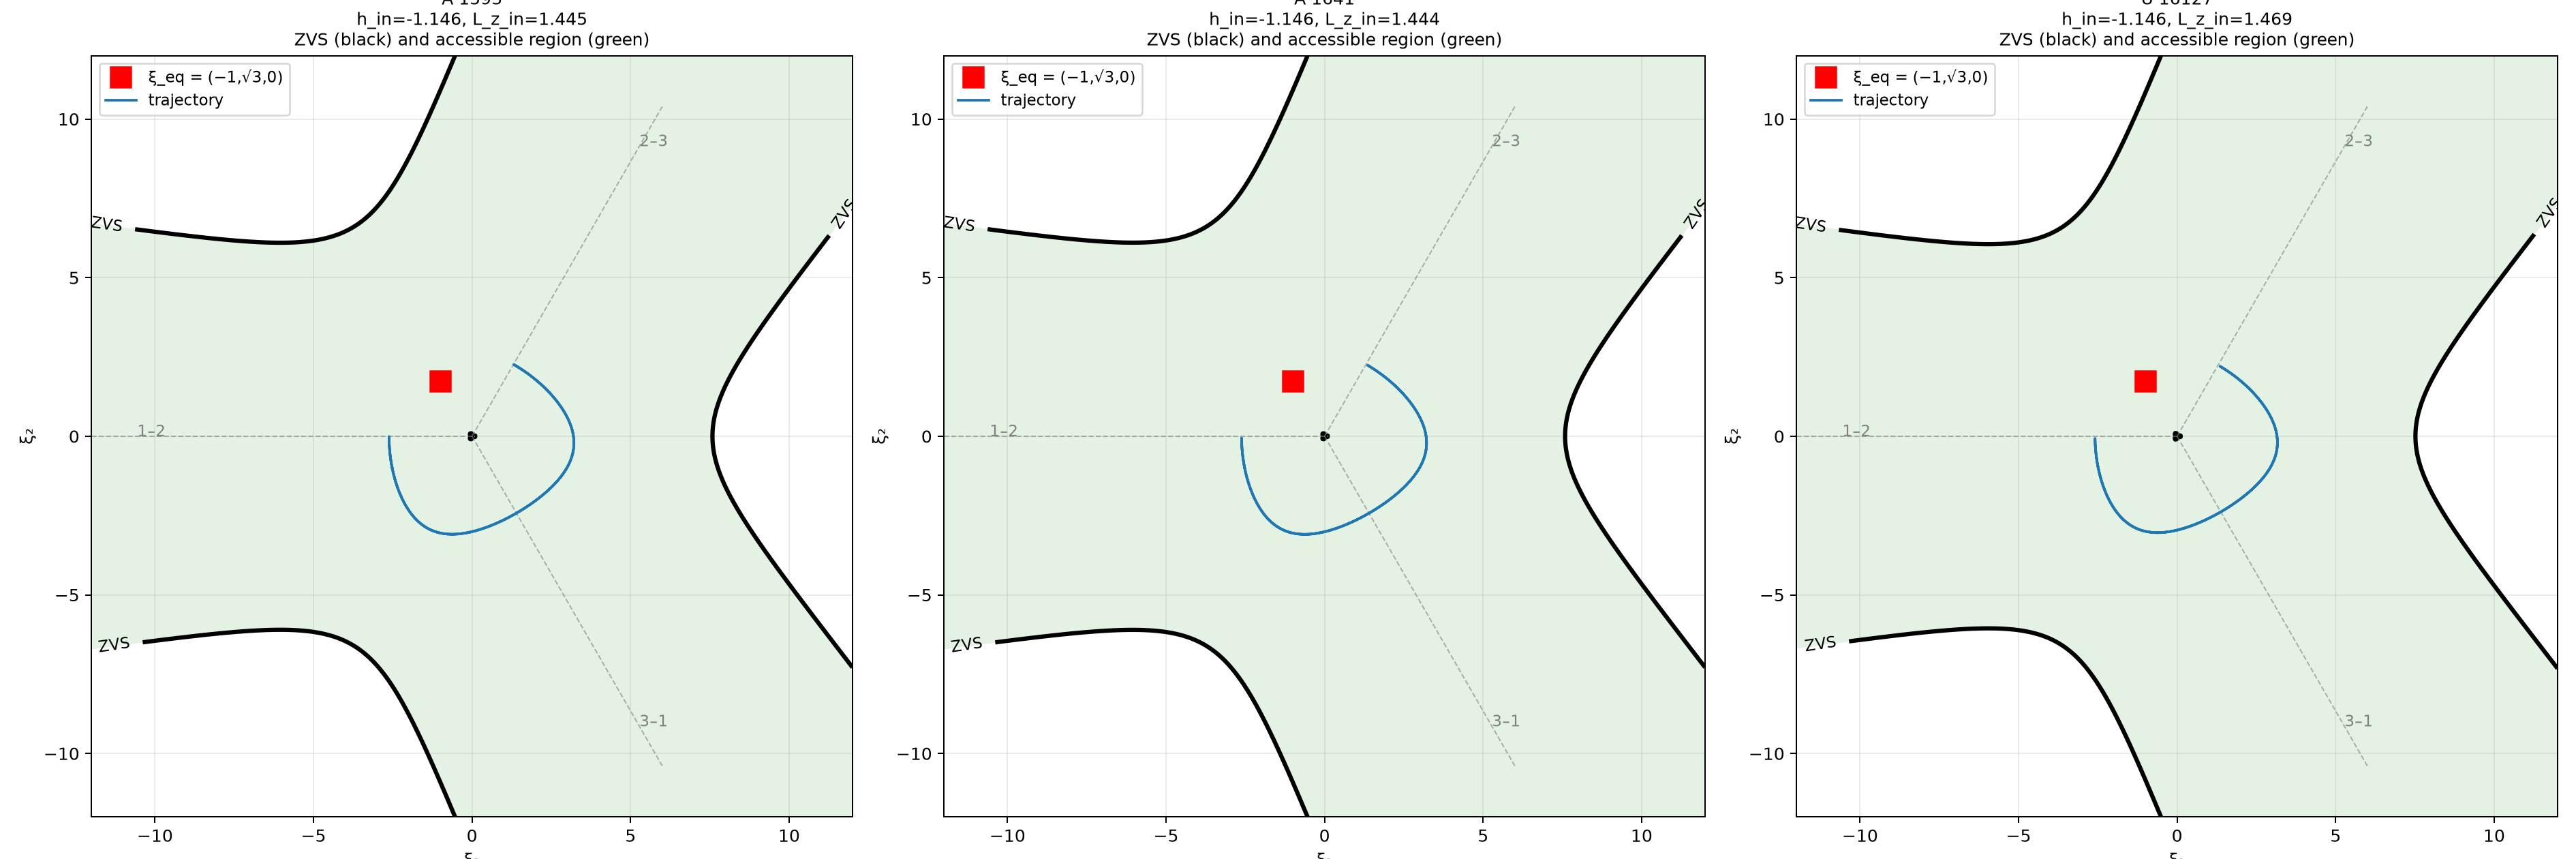
\includegraphics[width=\textwidth]{93_xi_zvs_xi3_0.png}
    \caption{Сечение поверхности нулевой скорости (ZVS) в плоскости \(\xi_3 = 0\) для трёх орбит (A 1593, A 1641, U 16127). Чёрная линия — ZVS; зелёным выделена доступная область; синяя линия — траектория орбиты. Лучи коллизий (пунктир) отмечены под углами \(\pi\), \(\pi/3\), \(-\pi/3\).}
    \label{fig:zvs_2d}
\end{figure}

3D-визуализация ZVS для орбиты A 1641 показана на рисунке~\ref{fig:zvs_3d}. Поверхность образует «капсулу» вокруг \(\xi_{eq}\), а «воронки», уходящие в бесконечность, соответствуют лучам столкновений (в них \(V \to -\infty\) и доступная область открывается). Траектория орбиты 1641 заключена внутри этой капсулы.

\begin{figure}[H]
    \centering
    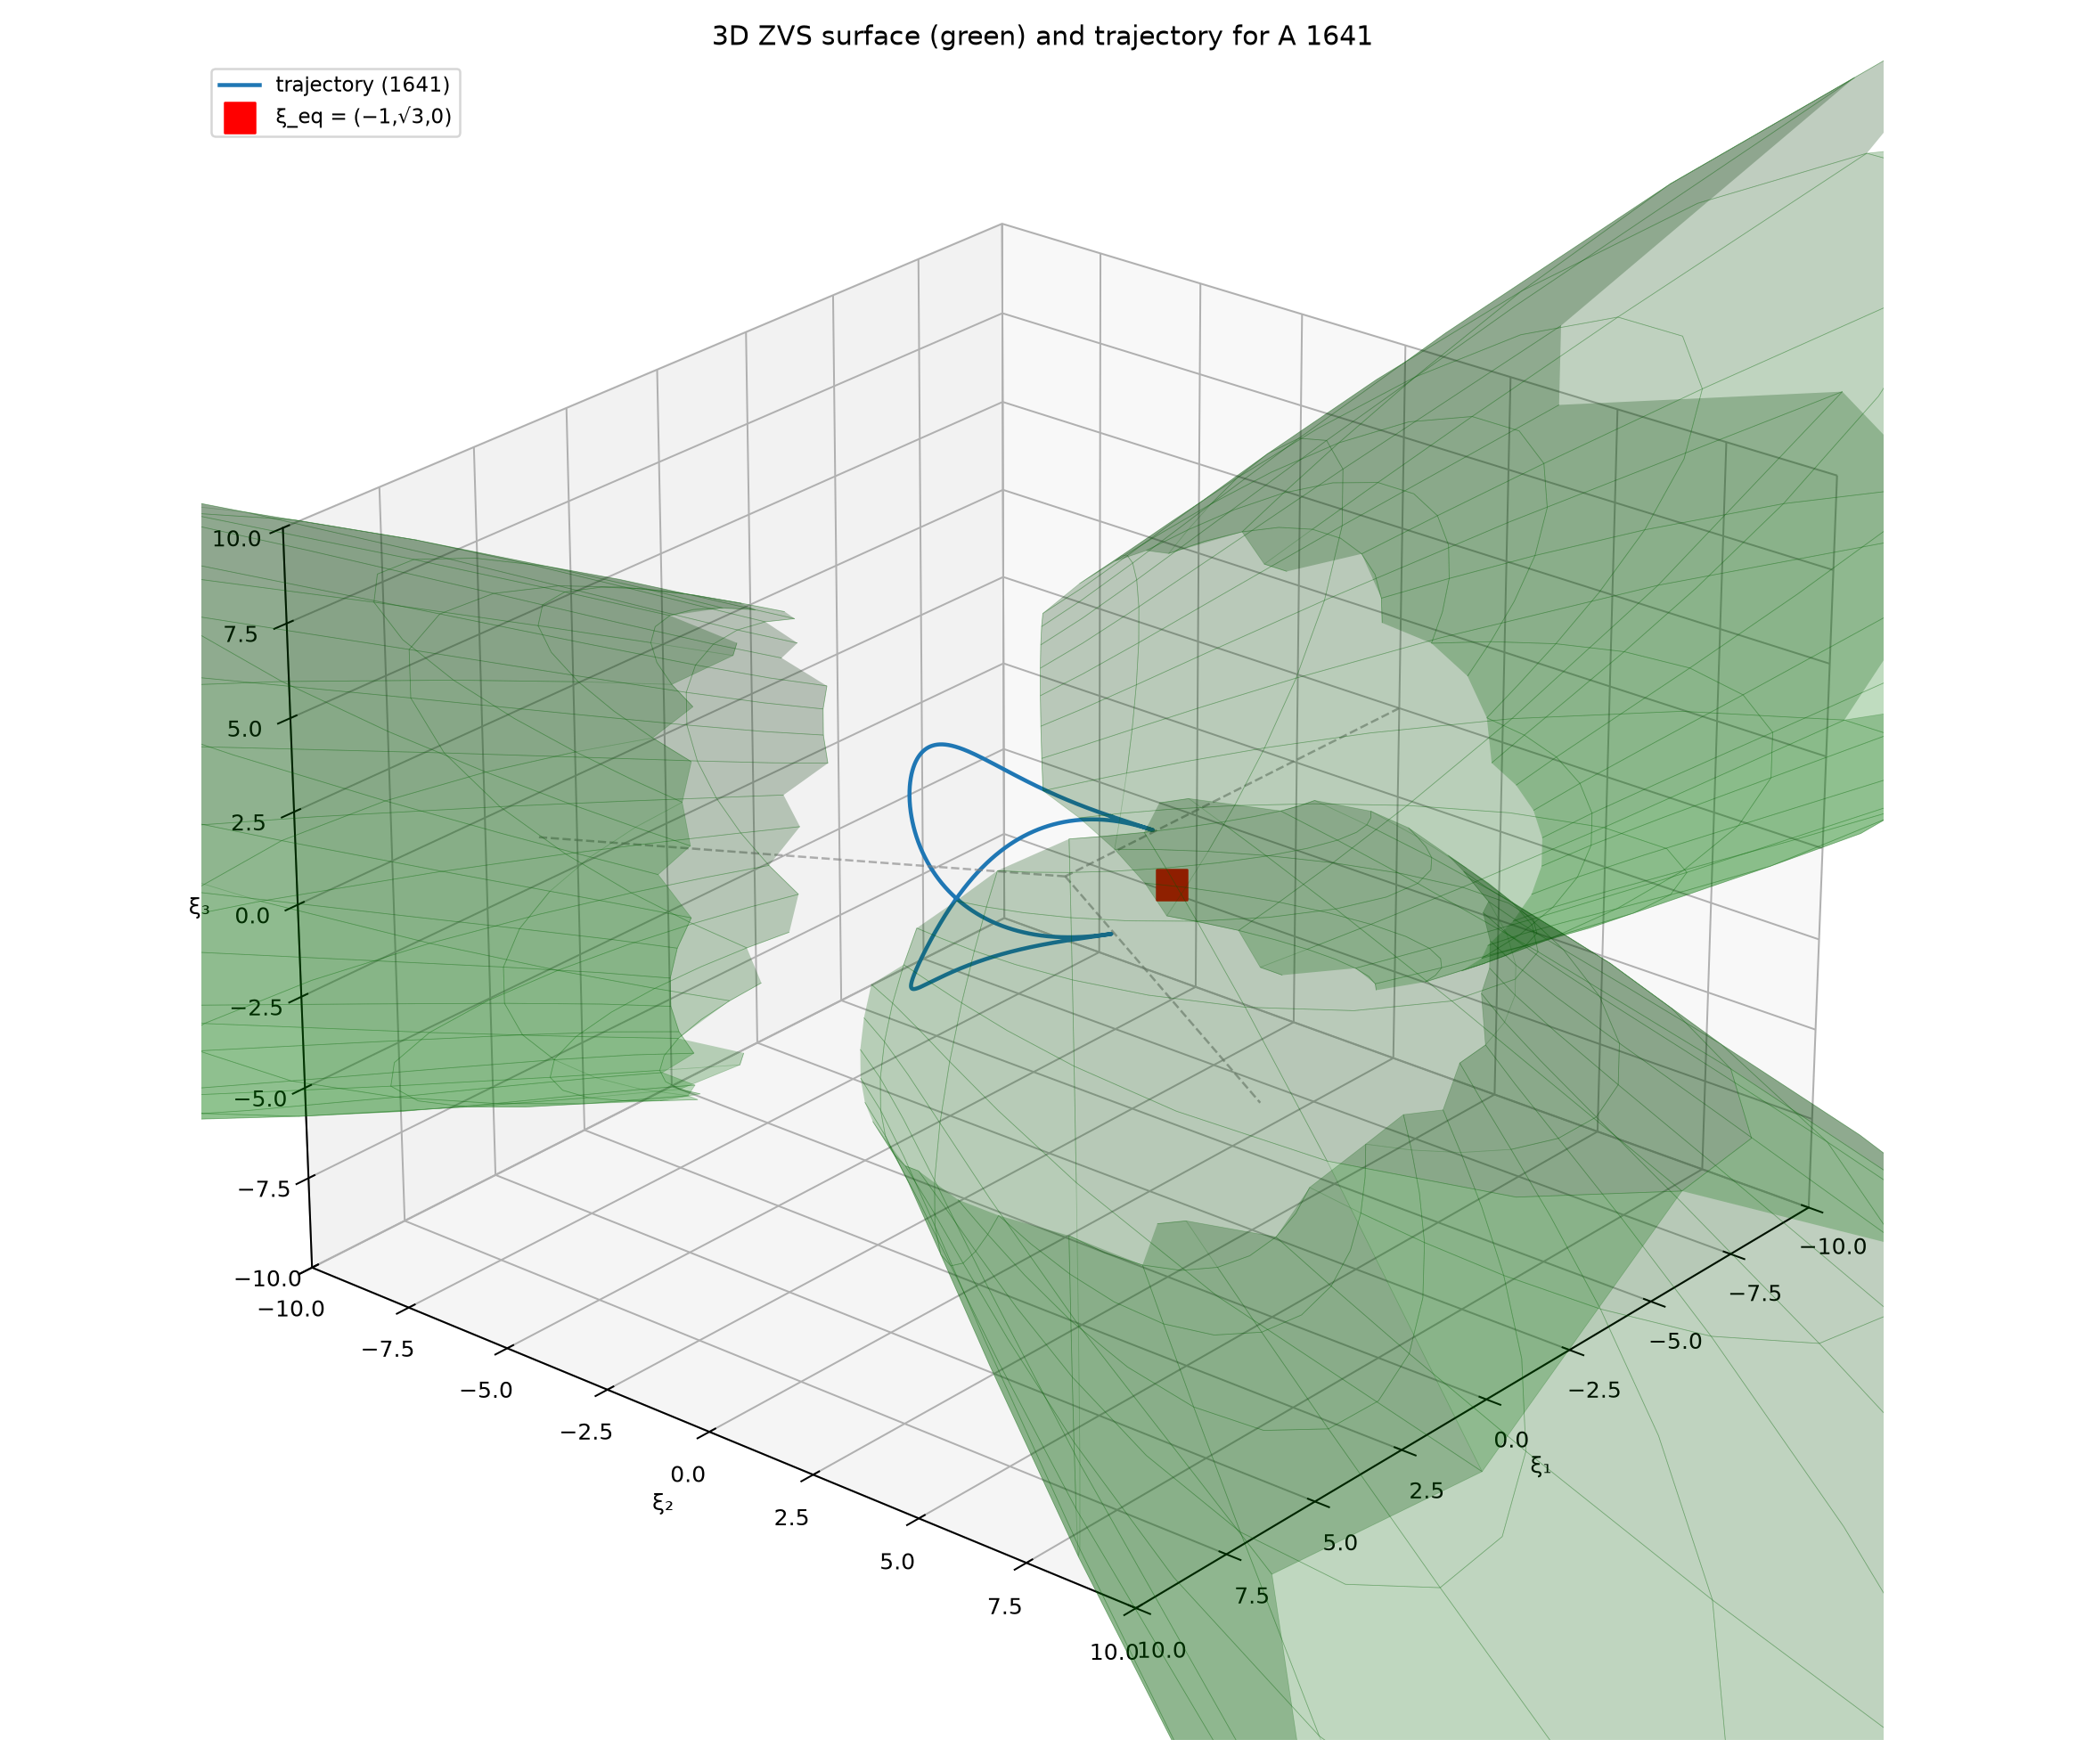
\includegraphics[width=0.85\textwidth]{93_xi_zvs_3d_1641.png}
    \caption{3D-визуализация поверхности нулевой скорости и траектории орбиты A 1641 в \(\xi\)-пространстве.}
    \label{fig:zvs_3d}
\end{figure}

\subsection{Запас по ZVS и отсутствие касания}
Количественно близость орбиты к ZVS характеризуется величиной
\begin{equation}
    \text{margin}(t) = h_{in} - V(\xi(t)) - \frac{L_z^2}{2|\xi(t)|},
\end{equation}
которая должна быть положительной для всех \(t\). Для всех проверенных орбит \(\min_t \text{margin}(t) > 0\) (обычно 1.5–2.4; минимальное значение \(\approx 1.1\) наблюдается около \(gidx \approx 15000\)). 

Графики \(\text{margin}(t)\) для трёх орбит (рисунок~\ref{fig:margin}) показывают, что запас положителен на всём периоде и имеет характерные пики в моменты сближений (там \(V\) резко возрастает по модулю, но не достигает \(h_{in}\)).

\begin{figure}[H]
    \centering
    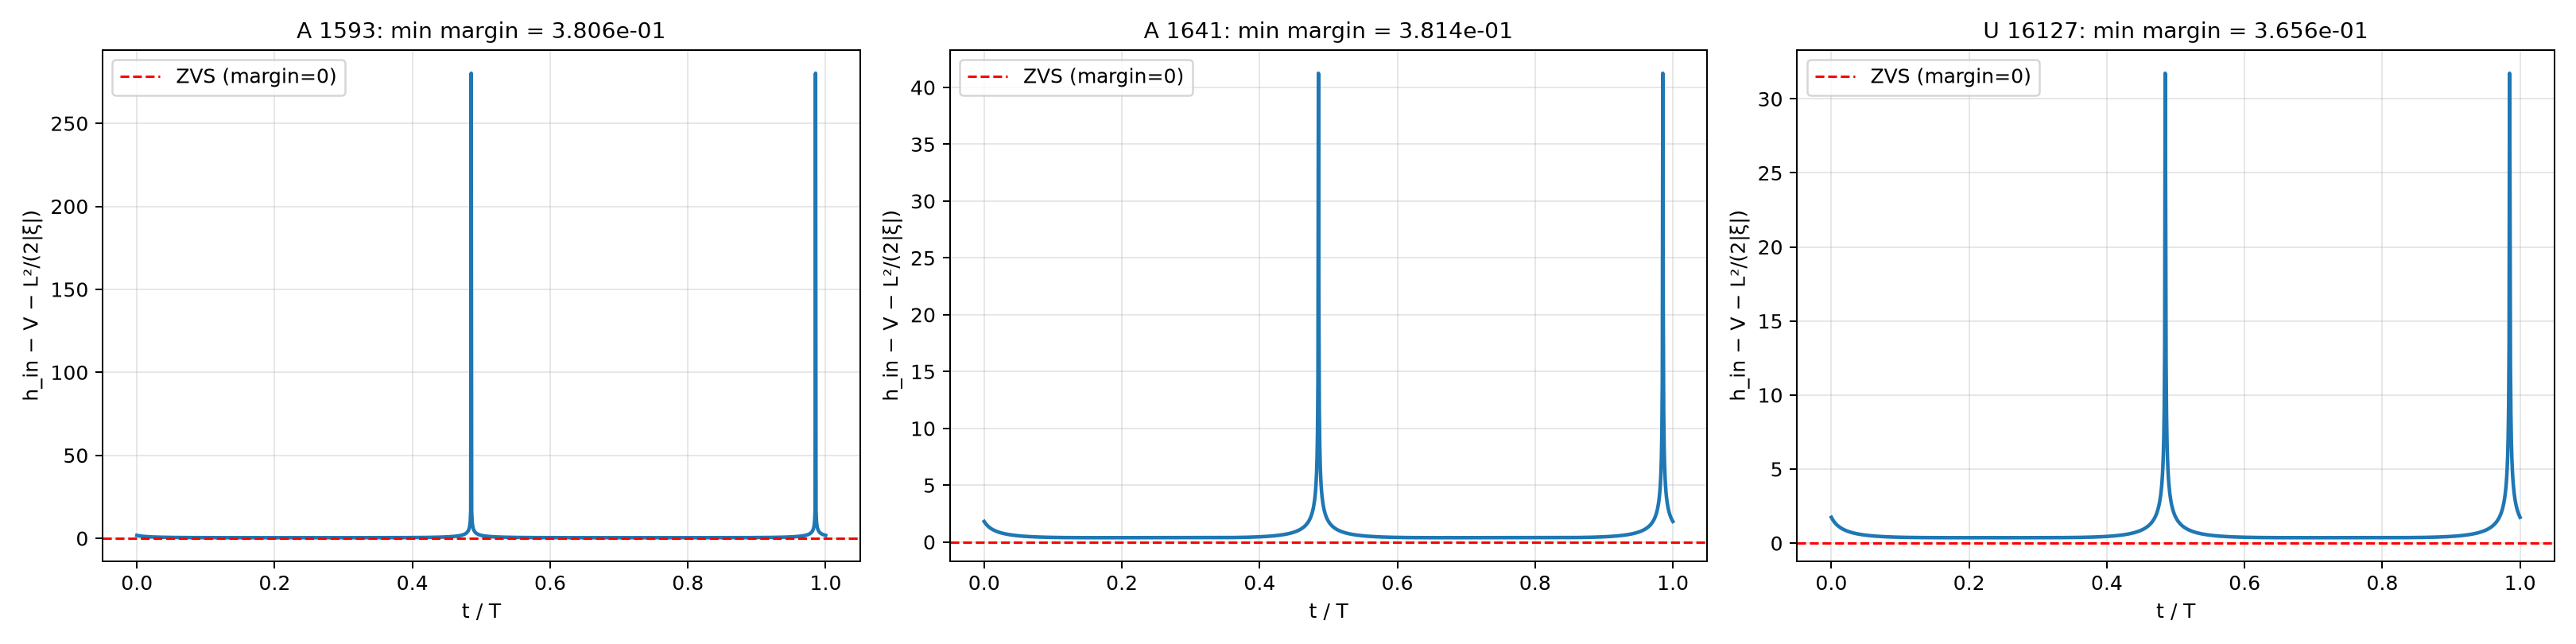
\includegraphics[width=\textwidth]{93_xi_margin.png}
    \caption{Запас \(\text{margin}(t) = h_{in} - V - L_z^2/(2|\xi|)\) вдоль траектории для трёх орбит. Красная линия — граница ZVS (\(\text{margin} = 0\)); она нигде не пересекается.}
    \label{fig:margin}
\end{figure}

\subsection{Вывод: ZVS не является механизмом переходов}
Совокупность результатов показывает: поверхность нулевой скорости \textbf{не является механизмом переходов} в этом семействе. Орбиты никогда не касаются ZVS, запас \(\text{margin}\) всюду положителен, а смена типа спектра (C \(\leftrightarrow\) R, OTHER \(\to\) C) происходит при значениях \(h_{in}\), далёких от критических. Ранее появлявшееся в скриптах сообщение о «переходе через ноль» было артефактом неверно заданных \(\xi_{eq}\) и углов коллизий, а также недостаточного сэмплирования.

\section{Численные эксперименты: геометрия и возмущения}

В предыдущих разделах устойчивость и топология орбит исследовались с помощью матрицы монодромии и координатных преобразований. В этом разделе мы приводим прямые численные эксперименты, которые, во-первых, показывают, как орбиты выглядят в инерциальной (абсолютной) системе отсчёта, а во-вторых, подтверждают, что вычисленный показатель Ляпунова \(\lambda\) действительно предсказывает скорость расхождения траекторий при малых начальных возмущениях.

\subsection{Орбиты в инерциальной системе отсчёта: розетки}
Состояния в каталогах записаны во вращающейся системе отсчёта. Для перехода в инерциальную систему необходимо учесть поворот на угол \(\Omega t\) (а для блока \textit{unified} — ещё и снять начальный поворот \(-\theta\), применённый в каталоге).

Если интегрировать орбиту в инерциальной системе ровно на один период \(T\), то траектория не замыкается: рамка вращается, и за период накапливается поворот на угол \(\Delta\varphi = \Omega T\). Для орбит блока \textit{arclength} отношение \(\Omega T / (2\pi) \approx 1.2452 \approx 5/4\), то есть за один период рамка делает \(1\frac{1}{4}\) оборота. Поэтому, чтобы получить замкнутую «розетку», необходимо собрать \(K\) копий одной и той же проинтегрированной траектории, каждая из которых повёрнута на угол \(k \cdot \Omega T\) (\(k = 0, \dots, K-1\)). Для \(5/4\) достаточно \(K=4\): накопленный поворот составит \(5\) полных оборотов, и роза замкнётся с точностью до \(0.4\%\). Такой подход позволяет избежать накопления ошибок интегрирования на длинных временах (что критично для неустойчивых орбит).

Для орбит блока \textit{canonical} отношение \(\Omega T / (2\pi) \approx 0.61\), поэтому «розетки» там нет — тела движутся по почти круговым орбитам, и достаточно интегрировать один оборот барицентра \(T_{rot} = 2\pi/\Omega\) с \(K=1\).

Результаты для нескольких репрезентативных орбит показаны на рисунке~\ref{fig:inertial_grid}. Видно, что орбиты блока \textit{arclength} (нижние панели) образуют характерные 5-лепестковые розетки, а орбиты \textit{canonical} (верхние панели) — почти круговые.

\begin{figure}[H]
    \centering
    \includegraphics[width=\textwidth]{93_inertial_grid_v4.png}
    \caption{Орбиты в инерциальной системе отсчёта. Верхний ряд: блок \textit{canonical} (интегрирование одного оборота барицентра, \(K=1\)). Нижние ряды: блок \textit{arclength} (сборка из \(K=4\) копий одного периода, 5-лепестковые розетки).}
    \label{fig:inertial_grid}
\end{figure}

Отдельно на рисунке~\ref{fig:U5000_unstable} показано, как выглядит неустойчивая орбита \(U\,5000\) (блок \textit{canonical}, \(\max|\mu| \approx 826\)) при интегрировании на 1, 2 и 3 периода. Уже на втором периоде видно, что тело 2 уходит из центра, а тела 1 и 3 сходят со своих почти круговых орбит — это прямое визуальное проявление неустойчивости.

\begin{figure}[H]
    \centering
    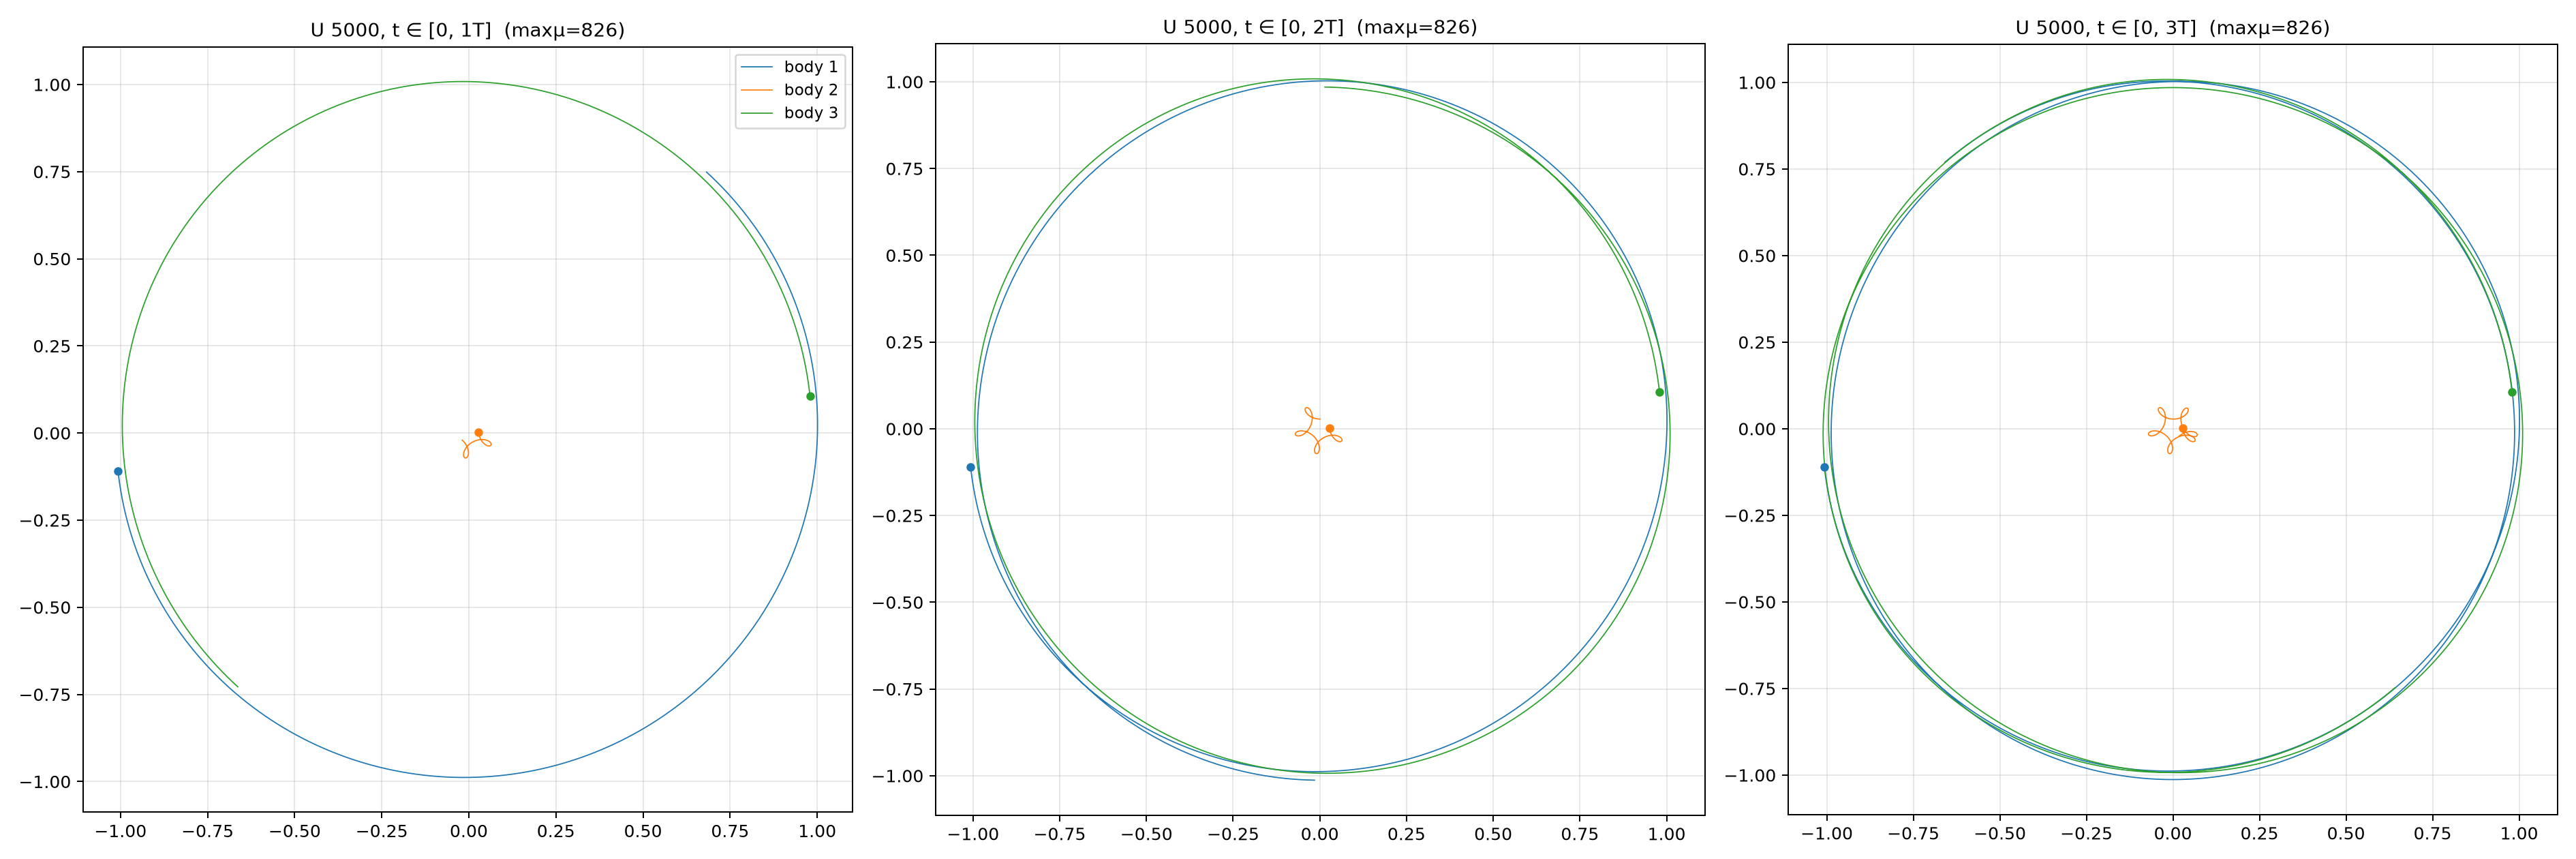
\includegraphics[width=\textwidth]{93d_U5000_1T_2T_3T.png}
    \caption{Неустойчивая орбита \(U\,5000\) в инерциальной системе при интегрировании на 1, 2 и 3 периода. Видно, как на втором периоде траектории начинают «разваливаться» из-за неустойчивости.}
    \label{fig:U5000_unstable}
\end{figure}

\subsection{Тесты на возмущение: рост \(| \Delta X(t) |\)}
Для прямой проверки связи между мультипликаторами Флоке и реальной скоростью расхождения траекторий был проведён следующий эксперимент. Берётся начальное состояние \(X_0\) из каталога и возмущённое состояние \(X_0 + \delta X\), где возмущение вносится только в координату \(y_1\): \(\delta y_1 = \delta\). Обе орбиты интегрируются на \(K\) периодов, и вычисляется евклидово расстояние в 8-мерном фазовом пространстве:
\begin{equation}
    |\Delta X(t)| = \| X(t; X_0) - X(t; X_0 + \delta X) \|.
\end{equation}
Согласно линейной теории, при малых \(\delta\) это расстояние должно расти как
\begin{equation}
    |\Delta X(t)| \approx C \cdot \delta \cdot e^{\lambda t}, \quad \lambda = \frac{\ln(\max|\mu|)}{T}.
\end{equation}
Коэффициент \(C\) зависит от того, насколько начальное возмущение \(\delta X\) «выровнено» по неустойчивому собственному вектору матрицы монодромии.

На рисунке~\ref{fig:pert_A1593} показаны результаты для орбиты \(A\,1593\) (блок \textit{arclength}). Слева — орбиты во вращающейся системе (исходная и возмущённая), в центре — \(| \Delta X(t) |\), справа — значения \(| \Delta X(nT) |\) в концах периодов и линейный фит. Видно, что \(\lambda_{\text{fit}} \approx 0.319\) практически совпадает с каталожным \(\lambda_{\text{cat}} \approx 0.324\). Это подтверждает, что вычисленный из матрицы монодромии показатель Ляпунова правильно предсказывает скорость расхождения траекторий.

\begin{figure}[H]
    \centering
    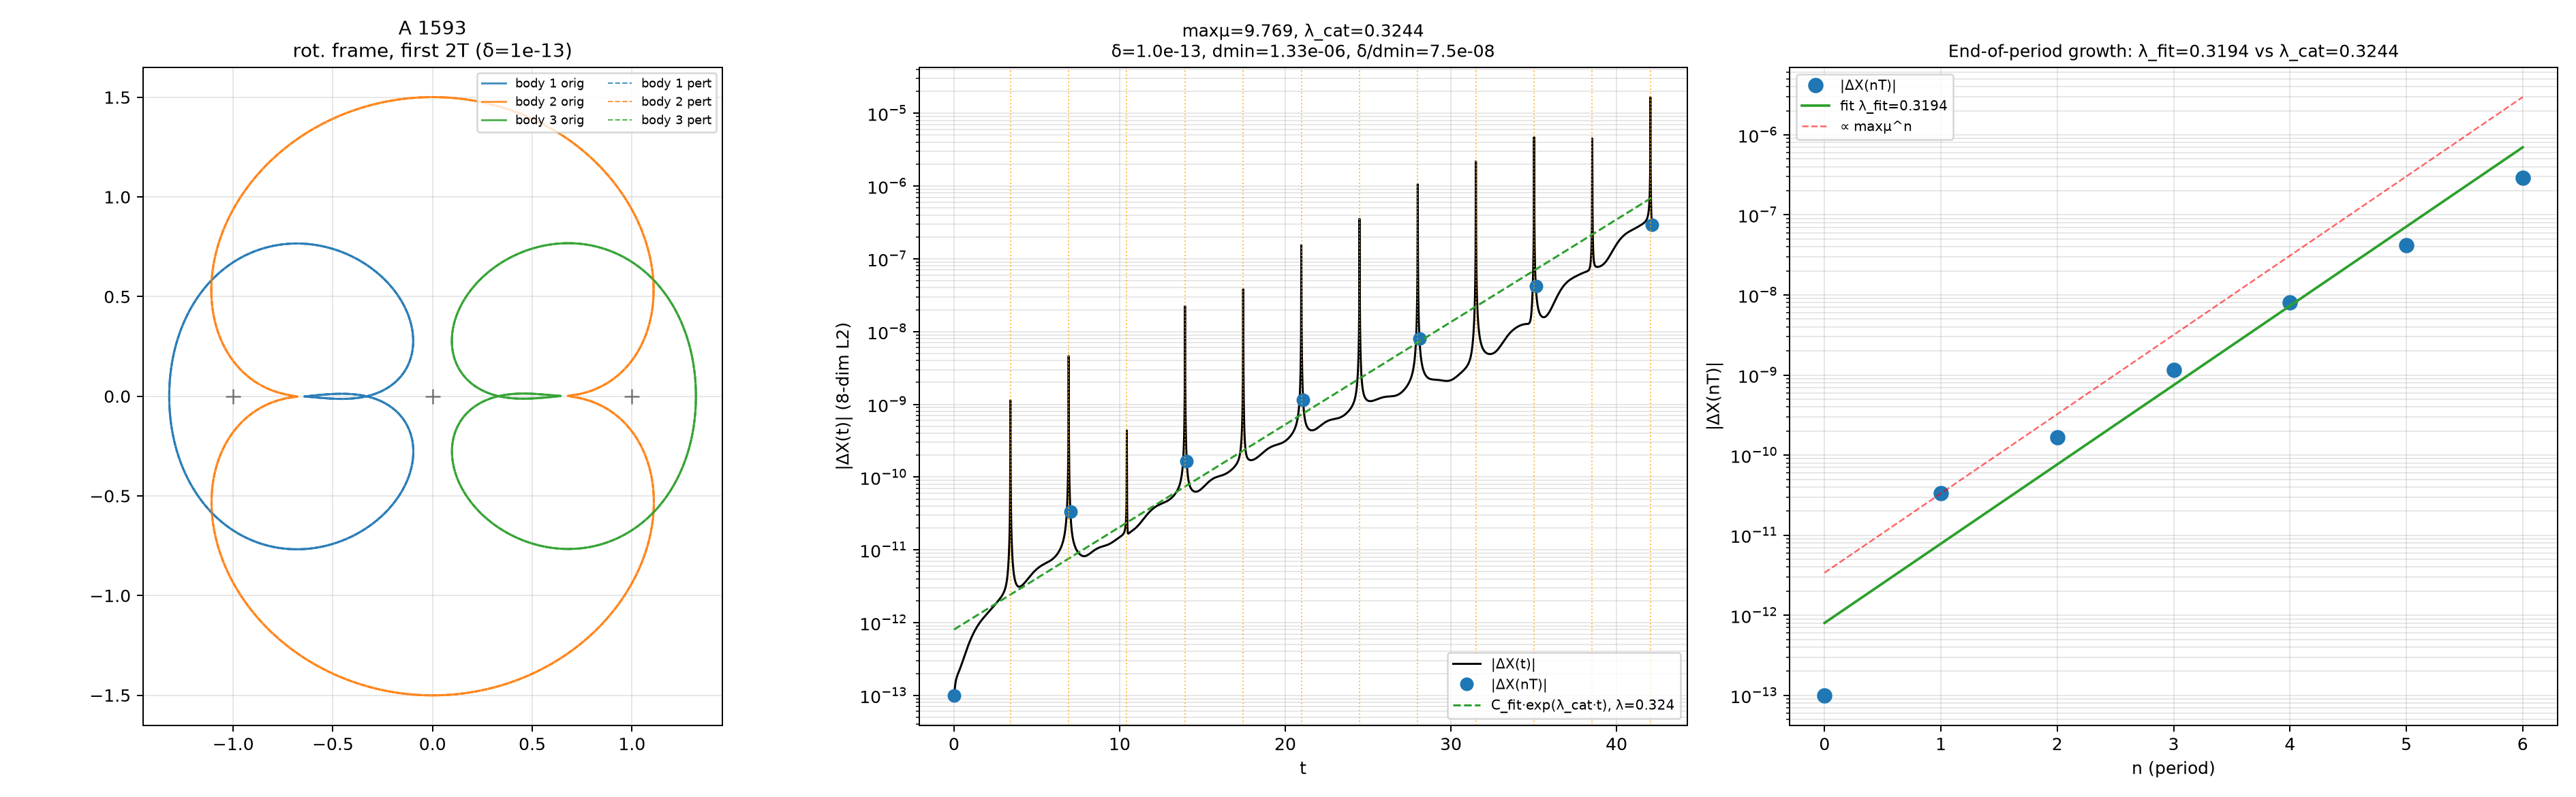
\includegraphics[width=\textwidth]{93_pert_A_1593.png}
    \caption{Тест на возмущение для орбиты \(A\,1593\) (\(\delta=10^{-13}\), \(K=6\)). Слева: орбиты во вращающейся системе (первые 2 периода). В центре: \(| \Delta X(t) |\). Справа: \(| \Delta X(nT) |\) и линейный фит \(\lambda_{\text{fit}} \approx 0.319\) (каталожное \(\lambda_{\text{cat}} \approx 0.324\)).}
    \label{fig:pert_A1593}
\end{figure}

Аналогичные результаты получены для орбиты \(A\,1641\) (рисунок~\ref{fig:pert_A1641}), где \(\lambda_{\text{fit}} \approx 0.381\) против \(\lambda_{\text{cat}} \approx 0.325\). Небольшое превышение объясняется нелинейными эффектами в моменты сближений (пики на центральной панели), но общий экспоненциальный закон выполняется.

\begin{figure}[H]
    \centering
    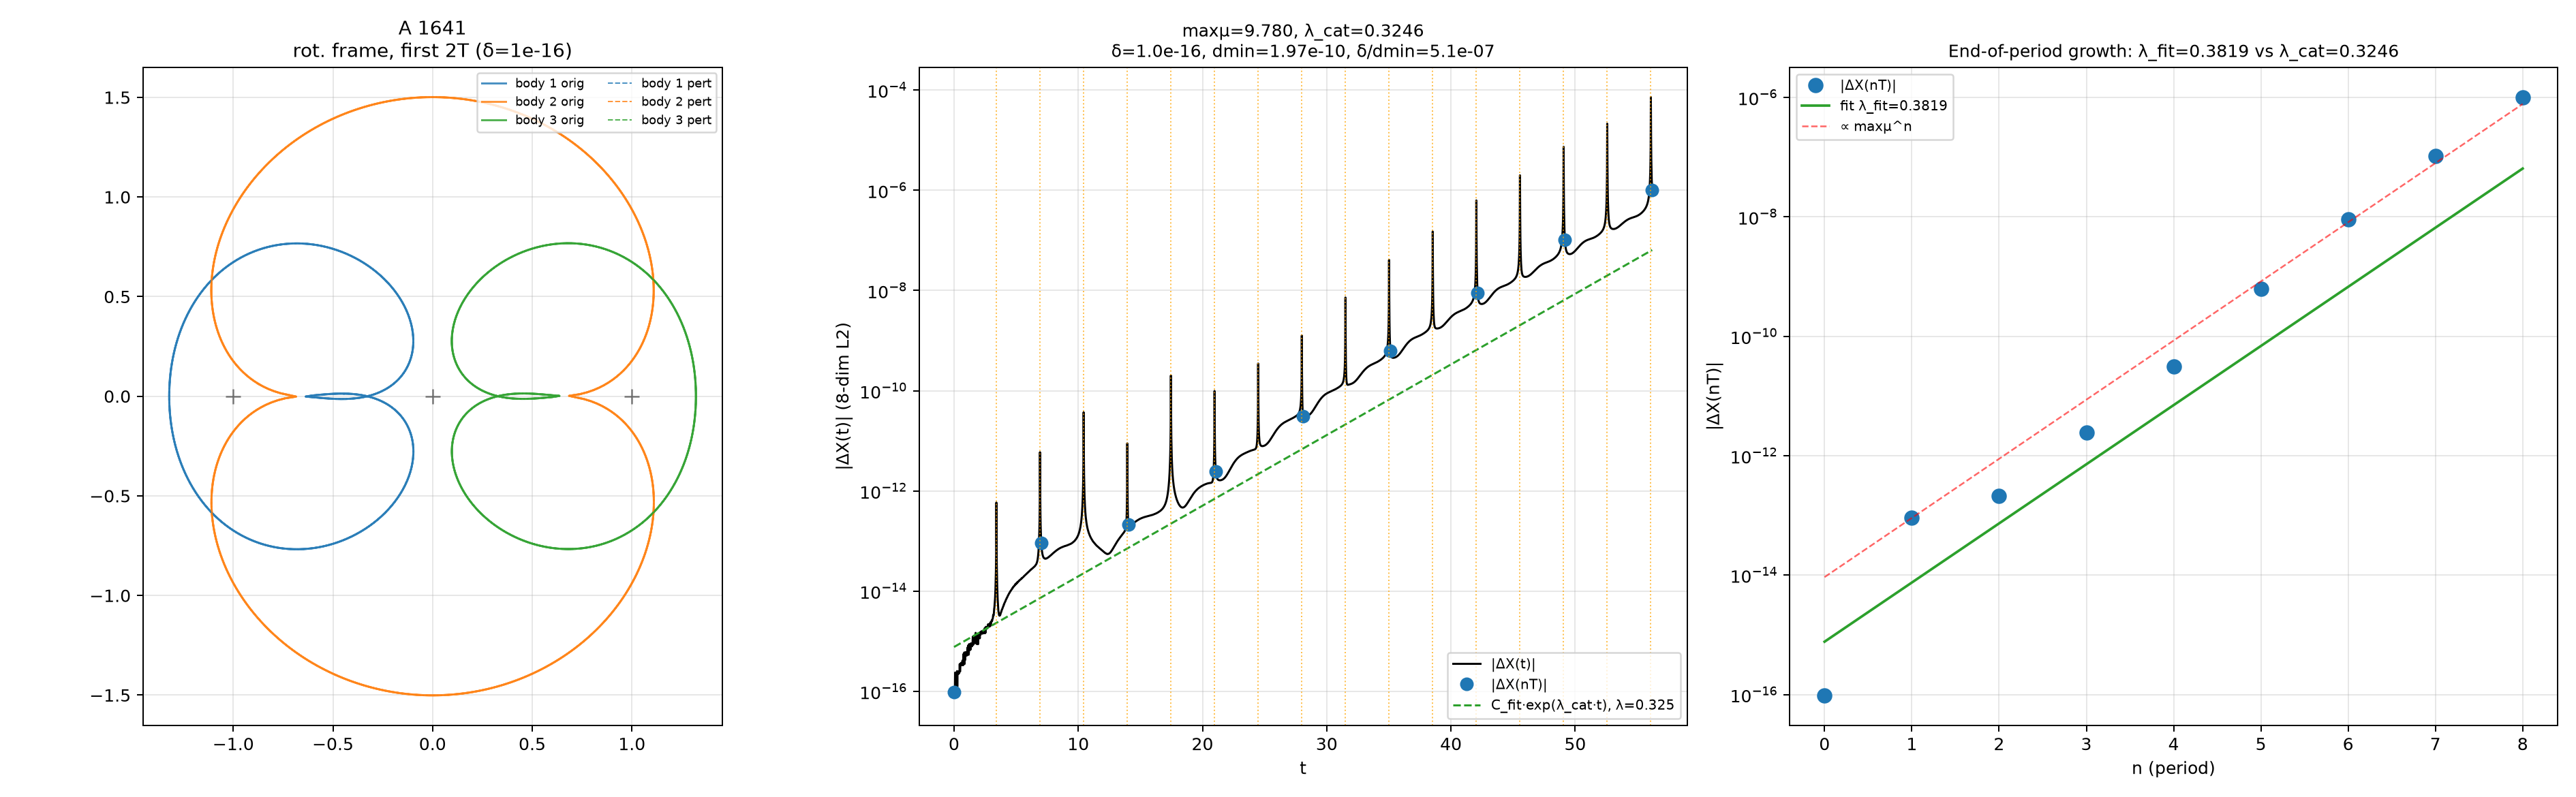
\includegraphics[width=\textwidth]{93_pert_A_1641.png}
    \caption{Тест на возмущение для орбиты \(A\,1641\) (\(\delta=10^{-16}\), \(K=8\)). \(\lambda_{\text{fit}} \approx 0.381\) против \(\lambda_{\text{cat}} \approx 0.325\).}
    \label{fig:pert_A1641}
\end{figure}

\subsection{Нелинейное насыщение на примере \(U\,5000\)}
Для сильно неустойчивой орбиты \(U\,5000\) (\(\max|\mu| \approx 826\), \(\lambda \approx 1.94\)) тест на возмущение демонстрирует важный нелинейный эффект: насыщение. При \(\delta = 10^{-7}\) возмущение растёт экспоненциально только до \(t \approx 9\), после чего \(| \Delta X(t) |\) выходит на плато \(\sim 10\) (рисунок~\ref{fig:pert_U5000}). Это происходит потому, что расстояние между двумя траекториями достигает размера всей фазовой области, и линейная теория перестаёт работать.

\begin{figure}[H]
    \centering
    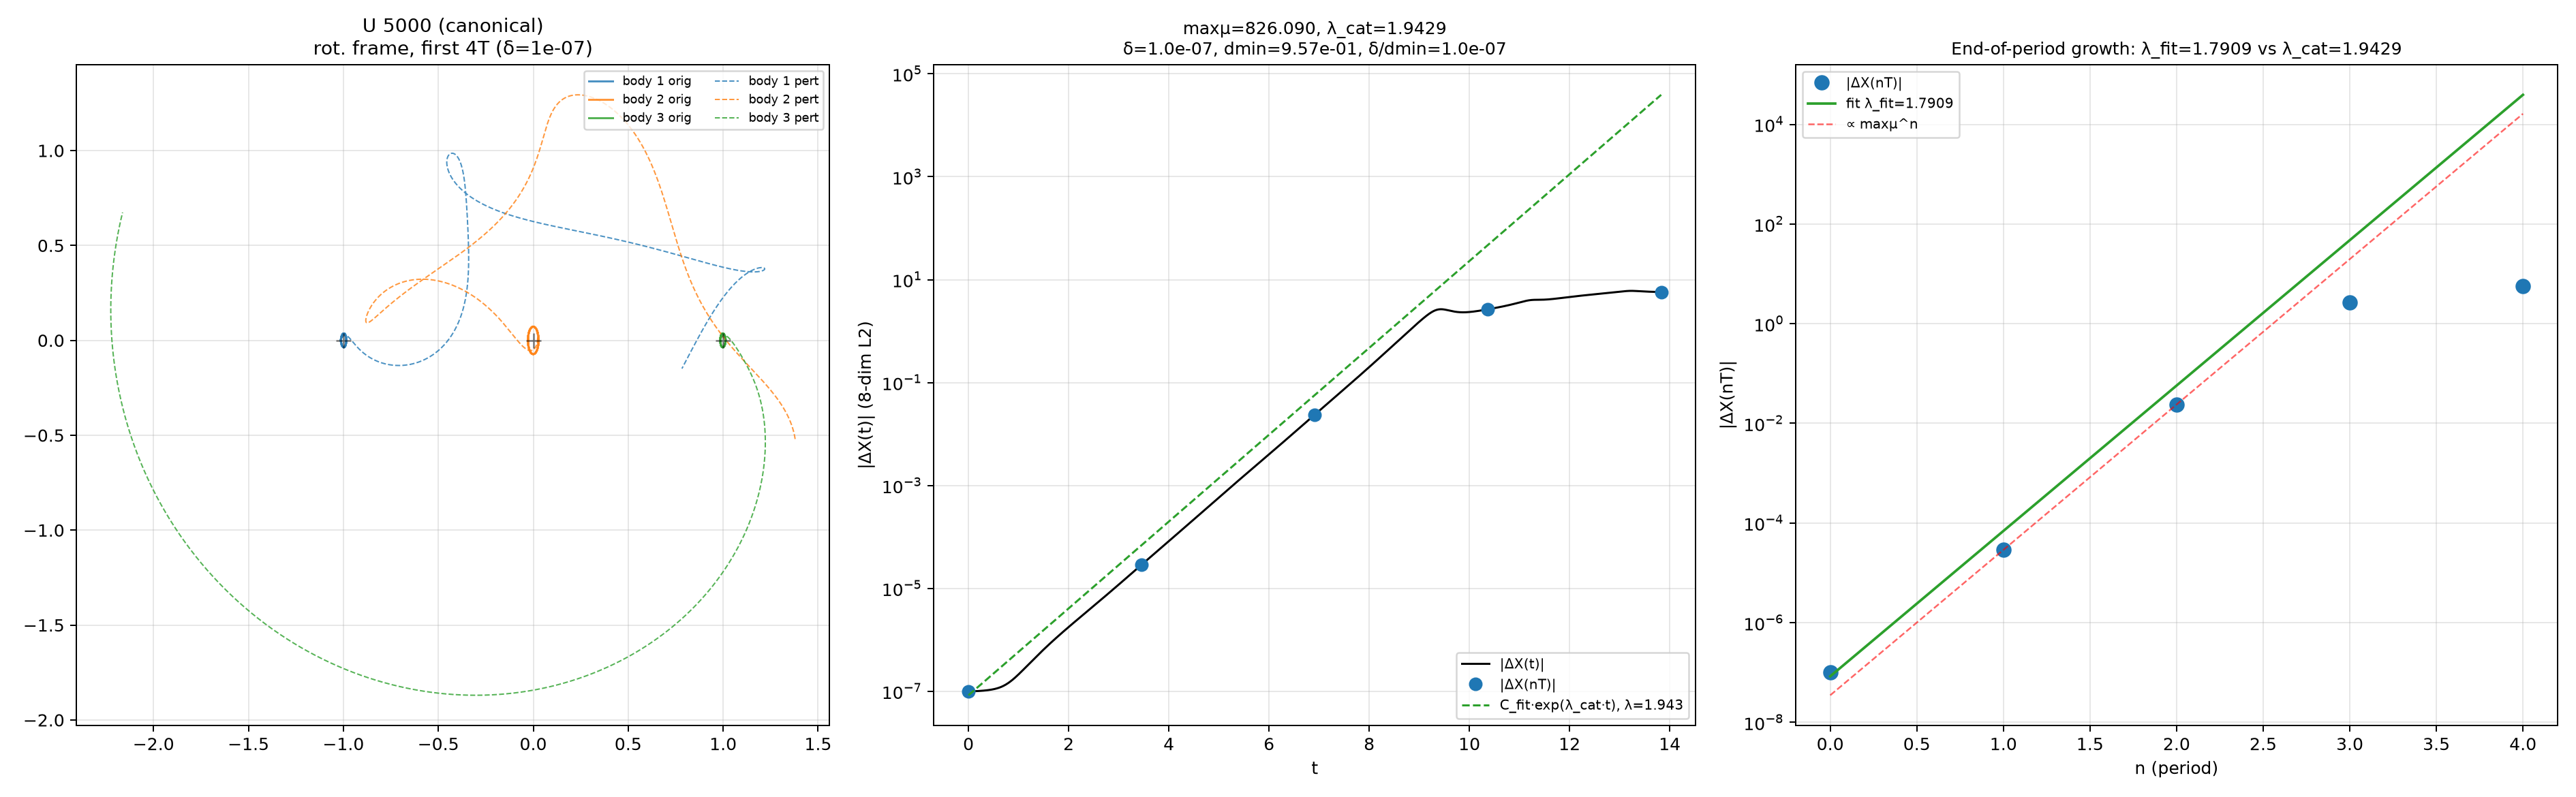
\includegraphics[width=\textwidth]{93_pert_U_5000.png}
    \caption{Тест на возмущение для орбиты \(U\,5000\) (\(\delta=10^{-7}\), \(K=4\)). Виден экспоненциальный рост \(| \Delta X(t) |\) до \(t \approx 9\) и последующее насыщение.}
    \label{fig:pert_U5000}
\end{figure}

Из-за насыщения линейный фит по всем 4 периодам даёт заниженное значение \(\lambda_{\text{fit}} \approx 1.79\) вместо \(\lambda_{\text{cat}} \approx 1.94\). Если же использовать только первые 2–3 периода (до насыщения), фит совпадает с теоретическим значением. Этот пример наглядно показывает границы применимости линейного анализа.

\subsection{Вывод по численным экспериментам}
Проведённые тесты подтверждают:
\begin{enumerate}
    \item Показатель Ляпунова \(\lambda = \ln(\max|\mu|)/T\), вычисленный из матрицы монодромии, правильно предсказывает скорость расхождения траекторий при малых возмущениях (для линейного режима \(\lambda_{\text{fit}} \approx \lambda_{\text{cat}}\)).
    \item На больших временах или при больших \(\delta\) проявляются нелинейные эффекты (насыщение), которые ограничивают применимость линейной теории.
    \item В инерциальной системе орбиты блока \textit{arclength} образуют 5-лепестковые розетки, что является геометрическим следствием отношения \(\Omega T/(2\pi) \approx 5/4\), а не резонансным захватом.
\end{enumerate}
% \input{sections/08_conclusion}

\end{document}
